% ============================================================
%  MedConnect – Rapport Technique Final
%  Groupe 12 – Web Services et Applications Distribuées
%  Structure calquée sur le rapport Atlas Trips (Équipe 8)
%  Compilé avec pdflatex (Overleaf)
% ============================================================
\documentclass[12pt,a4paper]{report}

% ── Encodage & langue ─────────────────────────────────────
\usepackage[utf8]{inputenc}
\usepackage[T1]{fontenc}
\usepackage{lmodern}
\usepackage[french]{babel}

% ── Mise en page ──────────────────────────────────────────
\usepackage[top=2.5cm,bottom=2.5cm,left=3cm,right=2.5cm]{geometry}

% ── Couleurs ──────────────────────────────────────────────
\usepackage[table,xcdraw]{xcolor}
\definecolor{medprimary}{HTML}{1a3c5e}
\definecolor{medsecondary}{HTML}{2980b9}
\definecolor{medaccent}{HTML}{e8f4fd}
\definecolor{medgray}{HTML}{f5f5f5}
\definecolor{medgreen}{HTML}{27ae60}
\definecolor{medred}{HTML}{c0392b}

% ── Tableaux ──────────────────────────────────────────────
\usepackage{booktabs}
\usepackage{tabularx}
\usepackage{longtable}
\usepackage{array}
\usepackage{multirow}
\usepackage{makecell}

% ── Graphiques & figures ───────────────────────────────────
\usepackage{graphicx}
\graphicspath{{screenshots/}{./}}
\usepackage{float}
\usepackage{caption}
\usepackage{subcaption}

% ── Code source ───────────────────────────────────────────
\usepackage{listings}
\lstset{
  basicstyle=\ttfamily\small,
  backgroundcolor=\color{medgray},
  frame=single,
  breaklines=true,
  columns=fullflexible,
  keepspaces=true,
  inputencoding=utf8,
  extendedchars=true,
  literate={é}{{\'e}}1 {è}{{\`e}}1 {ê}{{\^e}}1 {à}{{\`a}}1 {â}{{\^a}}1
           {ù}{{\`u}}1 {û}{{\^u}}1 {î}{{\^i}}1 {ô}{{\^o}}1 {ç}{{\c c}}1
}

% ── Mathématiques ─────────────────────────────────────────
\usepackage{amsmath}

% ── Listes ────────────────────────────────────────────────
\usepackage{enumitem}

% ── En-têtes & pieds de page ──────────────────────────────
\usepackage{fancyhdr}
\usepackage{lastpage}

\pagestyle{fancy}
\fancyhf{}
\renewcommand{\headrulewidth}{0.5pt}
\fancyhead[L]{\small\textcolor{medprimary}{\textbf{MedConnect}} – Rapport Technique}
\fancyhead[R]{\small Groupe 12}
\fancyfoot[C]{\small Page \thepage\ sur \pageref{LastPage}}

% ── Liens hypertexte ──────────────────────────────────────
\usepackage[hidelinks,
            pdftitle={MedConnect – Rapport Technique},
            pdfauthor={Groupe 12},
            pdfsubject={Web Services et Applications Distribuées}]{hyperref}

% ── Titres de sections ────────────────────────────────────
\usepackage{titlesec}
\titleformat{\chapter}[display]
  {\normalfont\huge\bfseries\color{medprimary}}
  {\chaptertitlename\ \thechapter}{20pt}{\Huge}
\titleformat{\section}
  {\normalfont\Large\bfseries\color{medprimary}}{\thesection}{1em}{}
\titleformat{\subsection}
  {\normalfont\large\bfseries\color{medsecondary}}{\thesubsection}{1em}{}
\titleformat{\subsubsection}
  {\normalfont\normalsize\bfseries}{\thesubsubsection}{1em}{}

% ── TikZ (diagrammes UML) ─────────────────────────────────
\usepackage{tikz}
\usetikzlibrary{shapes.geometric,shapes.multipart,arrows.meta,fit,positioning,calc,backgrounds}

% Styles UML réutilisables
\tikzset{
  % --- Use-case ---
  actor/.style={
    draw=medprimary, fill=medaccent, text=medprimary,
    ellipse, minimum width=2.2cm, minimum height=0.8cm,
    font=\small\bfseries, align=center
  },
  usecase/.style={
    draw=medsecondary, fill=white, text=black,
    ellipse, minimum width=3.2cm, minimum height=0.9cm,
    font=\small, align=center
  },
  actorbox/.style={
    draw=medprimary, fill=medprimary!10,
    rectangle, rounded corners=4pt,
    font=\small\bfseries\color{medprimary}, align=center,
    minimum width=2.4cm, minimum height=1cm
  },
  system/.style={
    draw=medprimary, thick, dashed, fill=medaccent!30,
    rectangle, rounded corners=6pt
  },
  % --- Classe ---
  classbox/.style={
    draw=medprimary, fill=white,
    rectangle split, rectangle split parts=3,
    rectangle split part fill={medprimary!80, white, white},
    font=\small, align=left,
    minimum width=3.8cm
  },
  inherit/.style={-{Triangle[open,length=8pt]}, draw=medprimary, thick},
  assoc/.style={-{Latex[length=6pt]}, draw=medsecondary, thick},
  comp/.style={-{Diamond[length=8pt]}, draw=medred, thick},
  % --- Composant ---
  compbox/.style={
    draw=medprimary, fill=medaccent, thick,
    rectangle, rounded corners=5pt,
    font=\small\bfseries\color{medprimary}, align=center,
    minimum width=3cm, minimum height=1.1cm
  },
  dbbox/.style={
    draw=medprimary, fill=medprimary!15, thick,
    cylinder, shape border rotate=90, aspect=0.15,
    font=\small\bfseries, align=center,
    minimum width=2.5cm, minimum height=1.2cm
  },
  nodebox/.style={
    draw=medprimary, fill=white, thick,
    rectangle, rounded corners=3pt,
    font=\small, align=center,
    minimum width=2.8cm, minimum height=0.9cm
  },
  serverbox/.style={
    draw=medsecondary, fill=medsecondary!10, thick,
    rectangle, rounded corners=5pt,
    font=\small\bfseries\color{medsecondary}, align=center,
    minimum width=4.5cm, minimum height=1.2cm
  },
  link/.style={-{Latex[length=5pt]}, draw=medprimary, thick},
  dlink/.style={-{Latex[length=5pt]}, draw=medsecondary, thick, dashed},
}

% ── Utilitaire ────────────────────────────────────────────
\usepackage{pdfpages}
\usepackage{pdflscape}
\setlength{\headheight}{15pt}

% ── Profondeur de la table des matières ───────────────────
\setcounter{tocdepth}{2}
\setcounter{secnumdepth}{3}

% ======================================================
\begin{document}
% ======================================================

% ══════════════════════════════════════════════════════
%  PAGE DE COUVERTURE
% ══════════════════════════════════════════════════════
\thispagestyle{empty}
\begin{titlepage}

  % En-tête institutionnel
  \begin{center}
    {\small ROYAUME DU MAROC}\\[0.3em]
    {\small Institut Supérieur de l'Information et de la Communication (ISIC)}\\[0.1em]
    \rule{\linewidth}{0.5pt}\\[0.5em]
    {\small Module : \textbf{Web Services et Applications Distribuées}}\\[0.2em]
    {\small Année universitaire 2026--2027}
  \end{center}

  \vspace{1.5cm}

  % Identité du groupe
  \begin{center}
    \colorbox{medprimary}{\parbox{0.6\textwidth}{\centering\vspace{0.4em}
      {\color{white}\Large\bfseries GROUPE 12}\\[0.2em]
    \vspace{0.3em}}}
  \end{center}

  \vspace{1cm}

  % Titre du projet
  \begin{center}
    {\color{medprimary}\rule{0.8\linewidth}{1.5pt}}\\[0.5em]
    {\Huge\bfseries\color{medprimary} MEDCONNECT}\\[0.4em]
    {\large\color{medsecondary} Plateforme Distribuée de Gestion de Cabinet Médical}\\[0.3em]
    {\color{medprimary}\rule{0.8\linewidth}{1.5pt}}
  \end{center}

  \vspace{0.8cm}

  % Sous-titre
  \begin{center}
    {\normalsize Rapport Technique Final}\\[0.2em]
    {\normalsize Référence : \texttt{MC-2026-RPT-001} \quad Version 1.0}\\[0.2em]
    {\normalsize Date : 23 novembre 2026}
  \end{center}

  \vspace{1cm}

  % Tableau équipe
  \begin{center}
  \renewcommand{\arraystretch}{1.4}
  \begin{tabular}{|p{4.5cm}|p{4.5cm}|p{5cm}|}
    \hline
    \rowcolor{medprimary}
    \textcolor{white}{\textbf{Nom}} &
    \textcolor{white}{\textbf{Rôle}} &
    \textcolor{white}{\textbf{Module responsable}} \\
    \hline
    Allabouch Anass & Chef de Projet & \texttt{patients\_api} \\
    \hline
    Ahmed Lahmaine & Product Owner / BA & \texttt{agenda\_api} \\
    \hline
    Achraf Ait Damnat & Lead Tech / Architecte & \texttt{dossier\_medical\_api} \\
    \hline
    Abdellah Rahel & QA / Conformité & \texttt{ordonnances\_api} \\
    \hline
  \end{tabular}
  \end{center}

  \vspace{0.8cm}

  \begin{center}
    {\normalsize Encadrant : \underline{\hspace{6cm}}}\\[1.5em]
    {\small\textit{23 novembre 2026}}
  \end{center}

\end{titlepage}

% ══════════════════════════════════════════════════════
%  FICHE D'IDENTIFICATION DU DOCUMENT
% ══════════════════════════════════════════════════════
\newpage
\thispagestyle{fancy}
\chapter*{Fiche d'Identification du Document}
\addcontentsline{toc}{chapter}{Fiche d'Identification du Document}

\renewcommand{\arraystretch}{1.4}

\begin{table}[H]
\centering
\caption{Identification du document}
\begin{tabular}{|p{5cm}|p{9cm}|}
  \hline
  \rowcolor{medaccent}
  \textbf{Champ} & \textbf{Valeur} \\
  \hline
  Nom du projet & MedConnect – Plateforme de Gestion de Cabinet Médical \\
  \hline
  Référence & MC-2026-RPT-001 \\
  \hline
  Version & 1.0 \\
  \hline
  Date & 23 novembre 2026 \\
  \hline
  Statut & \textcolor{medgreen}{\textbf{Validé}} \\
  \hline
  Équipe & Groupe 12 \\
  \hline
  Membres & Allabouch Anass, Ahmed Lahmaine, Achraf Ait Damnat, Abdellah Rahel \\
  \hline
  Responsable & Allabouch Anass (Chef de Projet) \\
  \hline
  Module & Web Services et Applications Distribuées \\
  \hline
  Dépôt GitHub & \texttt{github.com/AllabouchAnas/MedConnect-WS-IL-EQ12} \\
  \hline
  Branche principale & \texttt{main} \\
  \hline
\end{tabular}
\end{table}

\vspace{0.5cm}

\begin{table}[H]
\centering
\caption{Historique des versions}
\begin{tabular}{|c|c|p{3cm}|p{6cm}|}
  \hline
  \rowcolor{medaccent}
  \textbf{Version} & \textbf{Date} & \textbf{Auteur} & \textbf{Description} \\
  \hline
  0.1 & 01/11/2026 & Allabouch Anass & Architecture cible, structure du projet, \texttt{patients\_api} \\
  \hline
  0.2 & 08/11/2026 & Ahmed Lahmaine & \texttt{agenda\_api}, salle d'attente, gestion des RDV \\
  \hline
  0.3 & 15/11/2026 & Achraf Ait Damnat & \texttt{dossier\_medical\_api}, \texttt{ordonnances\_api} (Rahel) \\
  \hline
  1.0 & 23/11/2026 & Allabouch Anass & Consolidation finale, tests, rapport complet \\
  \hline
\end{tabular}
\end{table}

\vspace{0.5cm}

\noindent\textbf{Résumé :}\\
MedConnect est une plateforme web distribuée dédiée à la gestion de cabinets médicaux, développée en Python 3.14 avec Django REST Framework (DRF) et sécurisée par des jetons JWT. L'architecture repose sur quatre micro-services REST indépendants (\texttt{patients\_api}, \texttt{agenda\_api}, \texttt{dossier\_medical\_api}, \texttt{ordonnances\_api}) intégrés dans un monorepo Django, exposant des API conformes aux contraintes REST avec contrôle d'accès basé sur les rôles (RBAC). La base de données SQLite est utilisée en phase de développement, avec migration PostgreSQL prévue. La suite de tests couvre 68 cas (23 unitaires Pytest + 45 API Django), tous en succès.

\vspace{0.4cm}

\noindent\textbf{Mots-clés :} web services, REST, Django REST Framework, JWT, SQLite, cabinet médical, RBAC, Python, architecture distribuée, micro-services, Groupe 12.

% ══════════════════════════════════════════════════════
%  TABLE DES MATIÈRES
% ══════════════════════════════════════════════════════
\newpage
\tableofcontents

% ══════════════════════════════════════════════════════
%  LISTE DES FIGURES
% ══════════════════════════════════════════════════════
\newpage
\listoffigures
\listoftables

% ══════════════════════════════════════════════════════
%  SECTION 1 : INTRODUCTION
% ══════════════════════════════════════════════════════
\newpage
\chapter{Introduction}

\section{Contexte du projet}

Dans le cadre du module \textit{Web Services et Applications Distribuées}, le Groupe 12 a développé \textbf{MedConnect}, une plateforme web complète destinée à la gestion informatisée d'un cabinet médical. Le projet répond à une problématique réelle : la digitalisation des flux administratifs et médicaux au sein des cabinets de santé, notamment la gestion des patients, des rendez-vous, des dossiers médicaux et des ordonnances.

Le développement suit une architecture orientée services (SOA) où chaque fonctionnalité métier est encapsulée dans un service REST autonome. L'ensemble est construit sur Django REST Framework (DRF), un framework Python robuste et éprouvé pour la création d'API web conformes aux standards REST.

\section{Périmètre et acteurs}

Le périmètre fonctionnel de MedConnect couvre la gestion complète du cycle de vie d'un patient au sein d'un cabinet médical, depuis la prise de rendez-vous jusqu'à la remise d'une ordonnance. Deux acteurs principaux sont identifiés :

\renewcommand{\arraystretch}{1.4}
\begin{table}[H]
\centering
\caption{Acteurs du système MedConnect}
\begin{tabular}{|p{3.5cm}|p{10cm}|}
  \hline
  \rowcolor{medaccent}
  \textbf{Acteur} & \textbf{Responsabilités} \\
  \hline
  \textbf{Médecin} & Consultation des dossiers médicaux, rédaction et validation des ordonnances, gestion des consultations, accès complet à l'agenda \\
  \hline
  \textbf{Secrétaire} & Gestion des patients (CRUD), prise de rendez-vous, gestion de la salle d'attente, enregistrement des arrivées \\
  \hline
\end{tabular}
\end{table}

\section{Objectifs du projet}

Les objectifs fonctionnels et techniques du projet sont les suivants :

\begin{enumerate}[leftmargin=*, label=\textbf{O\arabic*.}]
  \item \textbf{Modularité} : Concevoir une architecture REST modulaire avec quatre services indépendants, chacun géré par un membre de l'équipe.
  \item \textbf{Sécurité} : Implémenter une authentification JWT et un contrôle d'accès RBAC différenciant médecin et secrétaire.
  \item \textbf{Couverture fonctionnelle} : Couvrir l'intégralité du cycle de vie d'un patient (inscription → RDV → consultation → ordonnance).
  \item \textbf{Qualité} : Atteindre 100\% de réussite sur la suite de tests (68 cas de test).
  \item \textbf{Maintenabilité} : Structurer le code pour faciliter la migration vers PostgreSQL et le déploiement Docker en V2.
\end{enumerate}

\section{Glossaire}

\begin{table}[H]
\centering
\caption{Glossaire des termes techniques}
\renewcommand{\arraystretch}{1.4}
\begin{tabular}{|p{3cm}|p{11cm}|}
  \hline
  \rowcolor{medaccent}
  \textbf{Terme} & \textbf{Définition} \\
  \hline
  \textbf{Patient} & Personne physique suivie par le cabinet, identifiée par son CIN \\
  \hline
  \textbf{CIN} & Carte d'Identité Nationale (identifiant unique du patient) \\
  \hline
  \textbf{RDV} & Rendez-vous médical planifié entre un patient et un médecin \\
  \hline
  \textbf{DME} & Dossier Médical Électronique – ensemble des consultations d'un patient \\
  \hline
  \textbf{JWT} & JSON Web Token – mécanisme d'authentification sans état (stateless) \\
  \hline
  \textbf{RBAC} & Role-Based Access Control – contrôle d'accès basé sur les rôles \\
  \hline
  \textbf{DRF} & Django REST Framework – bibliothèque Python pour la création d'API REST \\
  \hline
  \textbf{Ordonnance} & Document médical prescrivant des médicaments, immuable après validation \\
  \hline
  \textbf{Statut RDV} & État du rendez-vous : Planifié → Salle d'attente → En cours → Terminé / Annulé \\
  \hline
  \textbf{SimpleJWT} & Bibliothèque Django implémentant l'authentification JWT \\
  \hline
\end{tabular}
\end{table}

% ══════════════════════════════════════════════════════
%  SECTION 2 : BESOINS FONCTIONNELS
% ══════════════════════════════════════════════════════
\chapter{Besoins Fonctionnels et Règles de Gestion}

\section{Acteurs et cas d'utilisation}

Le tableau ci-dessous synthétise les fonctionnalités accessibles par acteur :

\begin{table}[H]
\centering
\caption{Matrice acteurs / fonctionnalités}
\renewcommand{\arraystretch}{1.4}
\begin{tabularx}{\textwidth}{|X|c|c|}
  \hline
  \rowcolor{medaccent}
  \textbf{Fonctionnalité} & \textbf{Médecin} & \textbf{Secrétaire} \\
  \hline
  Authentification (login / logout) & \checkmark & \checkmark \\
  \hline
  Gestion des patients (CRUD) & \checkmark (lecture) & \checkmark (complet) \\
  \hline
  Prise de rendez-vous & \checkmark & \checkmark \\
  \hline
  Annulation de rendez-vous & \checkmark & \checkmark \\
  \hline
  Gestion salle d'attente & \checkmark & \checkmark \\
  \hline
  Avancement statut RDV & \checkmark & \checkmark \\
  \hline
  Consultation dossier médical & \checkmark & \texttimes \\
  \hline
  Création de consultation & \checkmark & \texttimes \\
  \hline
  Rédaction d'ordonnance & \checkmark & \texttimes \\
  \hline
  Validation d'ordonnance & \checkmark & \texttimes \\
  \hline
  Visualisation des ordonnances & \checkmark & \texttimes \\
  \hline
\end{tabularx}
\end{table}

\section{Besoins fonctionnels par module}

\begin{longtable}{|p{3.5cm}|p{5cm}|p{5.5cm}|}
  \caption{Besoins fonctionnels et règles de gestion par module} \\
  \hline
  \rowcolor{medaccent}
  \textbf{Module} & \textbf{Besoin fonctionnel} & \textbf{Règle de gestion} \\
  \hline
  \endfirsthead
  \multicolumn{3}{l}{\small\textit{(suite du tableau)}} \\
  \hline
  \rowcolor{medaccent}
  \textbf{Module} & \textbf{Besoin fonctionnel} & \textbf{Règle de gestion} \\
  \hline
  \endhead
  \hline
  \endfoot

  \multirow{4}{*}{\textbf{patients\_api}} &
    Enregistrement d'un nouveau patient &
    CIN obligatoire et unique ; date de naissance validée \\
  \cline{2-3}
  & Mise à jour des informations & Secrétaire uniquement ; médecin en lecture seule \\
  \cline{2-3}
  & Recherche par CIN ou nom & Résultats paginés, tri par nom \\
  \cline{2-3}
  & Suppression logique & Désactivation (is\_active=False) sans suppression physique \\
  \hline

  \multirow{5}{*}{\textbf{agenda\_api}} &
    Création d'un RDV &
    Date/heure future obligatoire ; patient existant requis \\
  \cline{2-3}
  & Annulation d'un RDV & Statut → Annulé ; impossible si déjà Terminé \\
  \cline{2-3}
  & Avancement du statut & Flux strict : Planifié → Salle d'attente → En cours → Terminé \\
  \cline{2-3}
  & Salle d'attente & Liste des patients arrivés (statut = Salle d'attente) \\
  \cline{2-3}
  & Liste des médecins & Utilisateurs du groupe ``Medecin'' \\
  \hline

  \multirow{3}{*}{\textbf{dossier\_medical\_api}} &
    Création de consultation &
    Liée à un RDV en cours ; médecin uniquement \\
  \cline{2-3}
  & Historique des consultations & Trié par date décroissante ; lecture médecin \\
  \cline{2-3}
  & Détection des allergies & Alerte si médicament prescrit figure dans les allergies déclarées \\
  \hline

  \multirow{4}{*}{\textbf{ordonnances\_api}} &
    Création d'ordonnance &
    Liée à une consultation ; médecin uniquement \\
  \cline{2-3}
  & Ajout de lignes & Médicament + posologie ; vérification allergie automatique \\
  \cline{2-3}
  & Validation & Statut → validée ; immuable après validation \\
  \cline{2-3}
  & Visualisation & PDF ou JSON ; accessible médecin et secrétaire \\
  \hline
\end{longtable}

\section{Matrice RBAC}

\begin{table}[H]
\centering
\caption{Matrice de contrôle d'accès basé sur les rôles (RBAC)}
\renewcommand{\arraystretch}{1.4}
\begin{tabular}{|p{5cm}|c|c|c|}
  \hline
  \rowcolor{medaccent}
  \textbf{Endpoint / Ressource} & \textbf{Non auth.} & \textbf{Secrétaire} & \textbf{Médecin} \\
  \hline
  \texttt{POST /api/auth/login/} & \checkmark & \checkmark & \checkmark \\
  \hline
  \texttt{GET /api/patients/} & \texttimes & \checkmark & \checkmark \\
  \hline
  \texttt{POST /api/patients/} & \texttimes & \checkmark & \texttimes \\
  \hline
  \texttt{GET/POST /api/agenda/rdv/} & \texttimes & \checkmark & \checkmark \\
  \hline
  \texttt{POST /api/agenda/rdv/\{id\}/avancer/} & \texttimes & \checkmark & \checkmark \\
  \hline
  \texttt{GET /api/agenda/rdv/salle-attente/} & \texttimes & \checkmark & \checkmark \\
  \hline
  \texttt{GET /api/consultations/} & \texttimes & \texttimes & \checkmark \\
  \hline
  \texttt{POST /api/consultations/} & \texttimes & \texttimes & \checkmark \\
  \hline
  \texttt{GET/POST /api/ordonnances/} & \texttimes & \texttimes & \checkmark \\
  \hline
  \texttt{POST .../valider/} & \texttimes & \texttimes & \checkmark \\
  \hline
\end{tabular}
\end{table}

% ══════════════════════════════════════════════════════
%  SECTION 3 : MODÈLES UML
% ══════════════════════════════════════════════════════
\chapter{Modèles UML et Diagrammes}

\section{Diagramme de cas d'utilisation}

Le diagramme de cas d'utilisation représente les interactions entre les deux acteurs principaux (Secrétaire médicale et Médecin) et le système MedConnect, incluant les relations d'inclusion (\textit{«include»} pour la vérification des doublons et des chevauchements de créneaux) et d'extension (\textit{«extend»} pour l'ajout de pièces jointes à la consultation).

\begin{figure}[H]
\centering
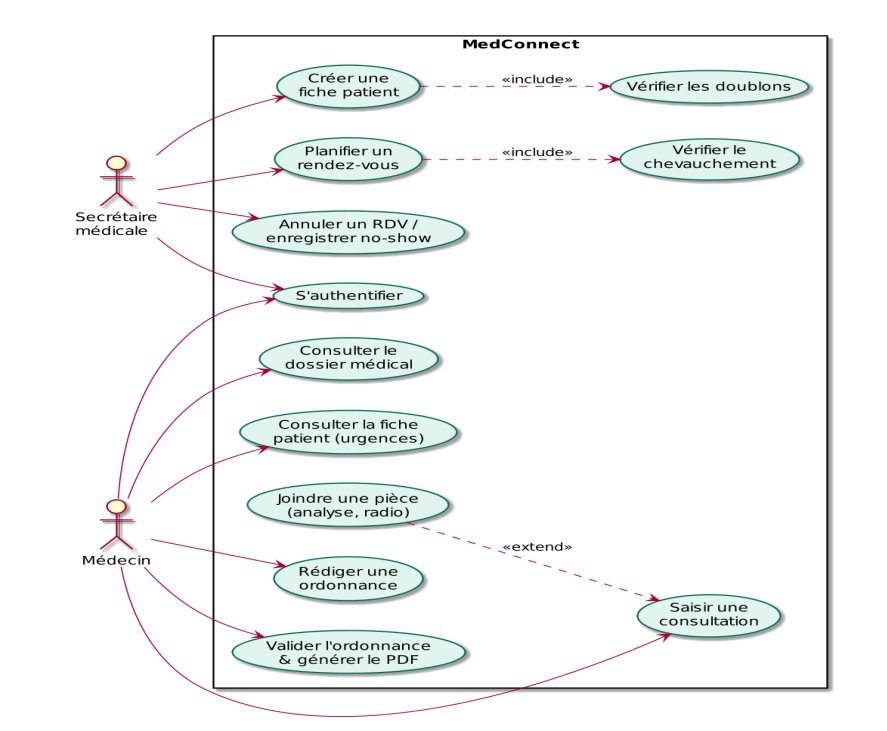
\includegraphics[width=0.88\textwidth]{uml_usecase.jpg}
\caption{Diagramme de cas d'utilisation – MedConnect}
\label{fig:uml-usecase}
\end{figure}

\section{Diagramme de classes}

Le diagramme de classes illustre le modèle conceptuel de données de la plateforme MedConnect, détaillant les entités métier (\texttt{Patient}, \texttt{Medecin}, \texttt{DossierMedical}, \texttt{RendezVous}, \texttt{Consultation}, \texttt{Ordonnance}, \texttt{LignePrescription}), leurs attributs, leurs opérations et les cardinalités des relations.

\begin{figure}[H]
\centering
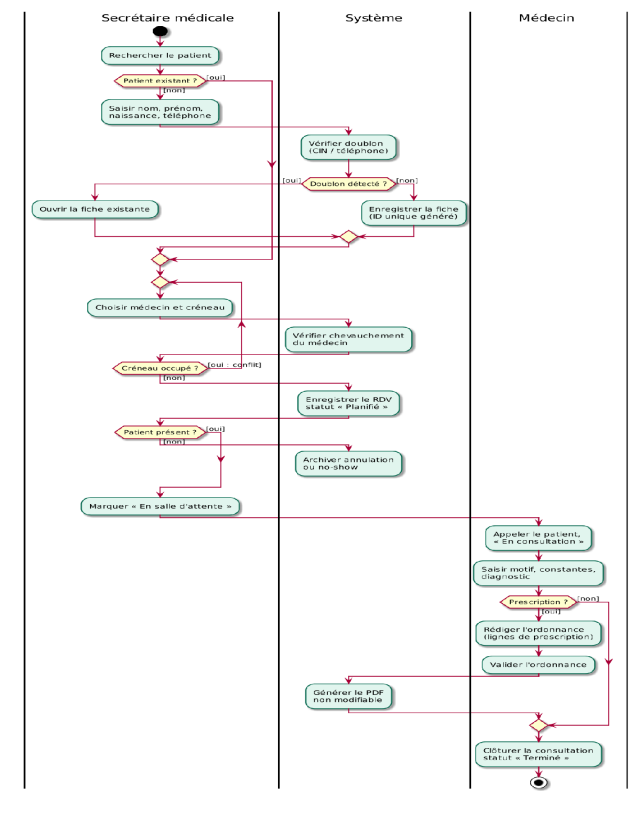
\includegraphics[width=\textwidth]{uml_classes.png}
\caption{Diagramme de classes – Modèle conceptuel et entités MedConnect}
\label{fig:uml-classes}
\end{figure}

\section{Diagramme d'activité – Flux métier et parcours patient}

Le diagramme d'activité en couloirs (\textit{swimlanes}) ci-après modélise l'enchaînement opérationnel entre la Secrétaire médicale, le Système MedConnect et le Médecin, depuis la recherche initiale du patient jusqu'à la clôture de la consultation et la génération de l'ordonnance non modifiable.

\begin{figure}[H]
\centering
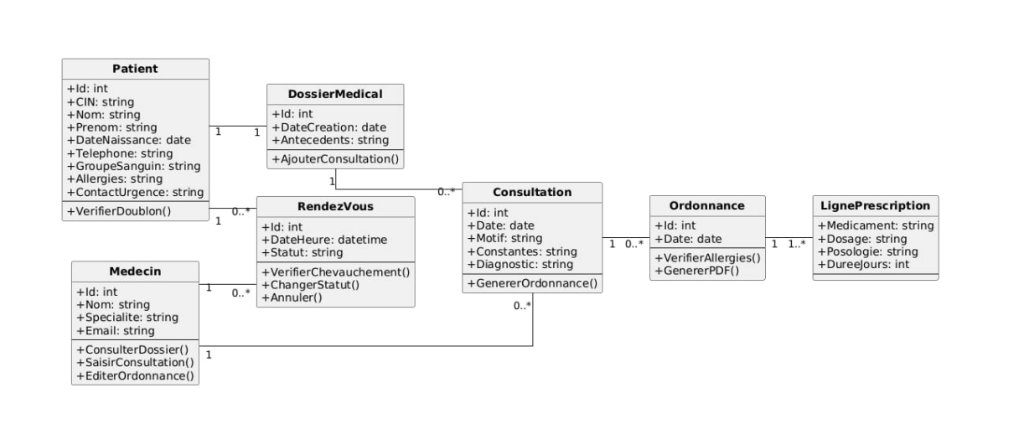
\includegraphics[width=0.82\textwidth]{uml_activite.jpg}
\caption{Diagramme d'activité – Parcours patient et flux de consultation}
\label{fig:uml-activite}
\end{figure}

\section{Diagramme de composants}

\begin{figure}[H]
\centering
\begin{tikzpicture}[node distance=1cm and 1.6cm]

  % ── Couche Client ─────────────────────────────
  \node[compbox, fill=medgreen!20, draw=medgreen, text=black, minimum width=10cm]
    (spa) {Frontend SPA\\{\small JavaScript ES6 + CSS3 – \texttt{fetch()} vers \texttt{/api/*}}};

  % ── Couche Gateway ────────────────────────────
  \node[compbox, below=0.9cm of spa, minimum width=10cm]
    (gw) {API Gateway – Django URL Dispatcher (\texttt{config/urls.py})\\{\small Routage vers les services + JWT middleware}};

  % ── Ligne Auth ────────────────────────────────
  \node[compbox, below left=1.2cm and -0.5cm of gw, minimum width=3cm, fill=medred!10, draw=medred]
    (auth) {auth\_service\\{\small SimpleJWT\\login / refresh / logout}};

  % ── 4 services ────────────────────────────────
  \node[compbox, right=0.4cm of auth] (p)   {patients\_api\\{\small PatientViewSet}};
  \node[compbox, right=0.4cm of p]    (ag)  {agenda\_api\\{\small RendezVousViewSet\\MedecinListView}};
  \node[compbox, right=0.4cm of ag]   (dm)  {dossier\_medical\_api\\{\small ConsultationViewSet}};
  \node[compbox, right=0.4cm of dm, minimum width=2.6cm]  (ord) {ordonnances\_api\\{\small OrdonnanceViewSet}};

  % ── ORM ───────────────────────────────────────
  \node[compbox, below=1.2cm of ag, minimum width=10cm, fill=medprimary!10]
    (orm) {Django ORM\\{\small models.py par service – migrations appliquées sur SQLite}};

  % ── BDD ───────────────────────────────────────
  \node[dbbox, below=0.9cm of orm, text width=2.5cm]
    (db) {SQLite 3\\db.sqlite3};

  % ── Liens ─────────────────────────────────────
  \draw[link] (spa)  -- (gw);
  \draw[link] (gw)   -- (auth);
  \draw[link] (gw)   -- (p);
  \draw[link] (gw)   -- (ag);
  \draw[link] (gw)   -- (dm);
  \draw[link] (gw)   -- (ord);
  \draw[link] (auth.south) |- (orm.west);
  \draw[link] (p.south)    -- (orm.north -| p.south);
  \draw[link] (ag.south)   -- (orm.north);
  \draw[link] (dm.south)   -- (orm.north -| dm.south);
  \draw[link] (ord.south)  |- (orm.east);
  \draw[link] (orm) -- (db);

  % ── Labels HTTP ───────────────────────────────
  \node[font=\tiny\itshape,color=medsecondary] at ($(spa)!0.5!(gw)+(3,0)$) {HTTP/REST JSON};
  \node[font=\tiny\itshape,color=medsecondary] at ($(orm)!0.5!(db)+(2,0)$) {SQL};

\end{tikzpicture}
\caption{Diagramme de composants – architecture MedConnect}
\label{fig:uml-composants}
\end{figure}

\section{Diagramme de séquence – Cycle de vie d'un RDV}

\begin{figure}[H]
\centering
\begin{tikzpicture}[node distance=0cm]

  % ── Lignes de vie ─────────────────────────────
  \node[nodebox] (sec)    at (0,0)    {Secrétaire};
  \node[nodebox] (client) at (3.5,0)  {Frontend\\SPA};
  \node[nodebox] (api)    at (7,0)    {Django API};
  \node[nodebox] (db)     at (10.5,0) {SQLite};
  \node[nodebox] (med)    at (14,0)   {Médecin};

  % traits de vie
  \foreach \x in {0,3.5,7,10.5,14} {
    \draw[draw=medprimary!40, dashed] (\x,-0.5) -- (\x,-12.5);
  }

  % ── Messages ──────────────────────────────────
  % 1. Création RDV
  \draw[link] (0,-1.0)  -- node[above,font=\tiny]{POST /api/agenda/rdv/} (7,-1.0);
  \draw[link] (7,-1.3)  -- node[above,font=\tiny]{INSERT RendezVous} (10.5,-1.3);
  \draw[dlink](10.5,-1.6) -- node[above,font=\tiny]{201 Created} (7,-1.6);
  \draw[dlink](7,-1.9)  -- node[above,font=\tiny]{statut=Planifié} (0,-1.9);

  \node[font=\tiny\bfseries\color{medprimary}] at (-1.2,-1.4) {RDV planifié};

  % 2. Arrivée patient
  \draw[link] (0,-2.8)  -- node[above,font=\tiny]{POST /api/agenda/rdv/\{id\}/avancer/} (7,-2.8);
  \draw[link] (7,-3.1)  -- node[above,font=\tiny]{UPDATE statut='Salle d'attente'} (10.5,-3.1);
  \draw[dlink](10.5,-3.4) -- node[above,font=\tiny]{200 OK} (7,-3.4);
  \draw[dlink](7,-3.7)  -- node[above,font=\tiny]{statut=Salle d'attente} (0,-3.7);

  \node[font=\tiny\bfseries\color{medprimary}] at (-1.2,-3.2) {Arrivée};

  % 3. Consultation
  \draw[link] (14,-4.6) -- node[above,font=\tiny]{POST /api/agenda/rdv/\{id\}/avancer/} (7,-4.6);
  \draw[link] (7,-4.9)  -- node[above,font=\tiny]{UPDATE statut='Consultation'} (10.5,-4.9);
  \draw[dlink](10.5,-5.2) -- node[above,font=\tiny]{200 OK} (7,-5.2);
  \draw[dlink](7,-5.5)  -- node[above,font=\tiny]{statut=Consultation} (14,-5.5);

  \node[font=\tiny\bfseries\color{medprimary}] at (15.3,-5.0) {Consultation};

  % 4. Création dossier médical
  \draw[link] (14,-6.4) -- node[above,font=\tiny]{POST /api/consultations/} (7,-6.4);
  \draw[link] (7,-6.7)  -- node[above,font=\tiny]{INSERT Consultation} (10.5,-6.7);
  \draw[dlink](10.5,-7.0) -- node[above,font=\tiny]{201 Created} (7,-7.0);
  \draw[dlink](7,-7.3)  -- node[above,font=\tiny]{consultation\_id} (14,-7.3);

  % 5. Ordonnance
  \draw[link] (14,-8.2) -- node[above,font=\tiny]{POST /api/ordonnances/ + ajouter-ligne} (7,-8.2);
  \draw[link] (7,-8.5)  -- node[above,font=\tiny]{INSERT Ordonnance + LigneOrdonnance} (10.5,-8.5);
  \draw[dlink](10.5,-8.8) -- node[above,font=\tiny]{201 Created} (7,-8.8);
  \draw[dlink](7,-9.1)  -- node[above,font=\tiny]{ordonnance\_id} (14,-9.1);

  % 6. Validation ordonnance
  \draw[link] (14,-10.0)-- node[above,font=\tiny]{POST /api/ordonnances/\{id\}/valider/} (7,-10.0);
  \draw[link] (7,-10.3) -- node[above,font=\tiny]{UPDATE est\_validee=True} (10.5,-10.3);
  \draw[dlink](10.5,-10.6)-- node[above,font=\tiny]{200 OK} (7,-10.6);

  % 7. Clôture RDV
  \draw[link] (14,-11.5)-- node[above,font=\tiny]{POST /api/agenda/rdv/\{id\}/avancer/} (7,-11.5);
  \draw[link] (7,-11.8) -- node[above,font=\tiny]{UPDATE statut='Terminé'} (10.5,-11.8);
  \draw[dlink](10.5,-12.1)-- node[above,font=\tiny]{200 OK – statut=Terminé} (7,-12.1);

  \node[font=\tiny\bfseries\color{medgreen}] at (15.3,-11.8) {Terminé};

\end{tikzpicture}
\caption{Diagramme de séquence – cycle de vie complet d'un rendez-vous médical}
\label{fig:uml-sequence}
\end{figure}

\section{Diagramme de déploiement}

\begin{figure}[H]
\centering
\begin{tikzpicture}[node distance=1.2cm and 2cm]

  % ── Nœud Poste Client ─────────────────────────
  \node[serverbox, minimum width=5.5cm, minimum height=2.4cm, label={[font=\small\bfseries]above:«node» Poste Client}]
    (client_node) at (0,0) {};
  \node[nodebox, fill=medgreen!10] (browser) at (0,0) {Navigateur Web\\{\small Chrome / Firefox / Edge}};
  \node[nodebox, fill=medgreen!10, below=0.3cm of browser] (spa_art) {{\small \texttt{index.html + JS/CSS SPA}}};

  % ── Nœud Serveur Django ───────────────────────
  \node[serverbox, minimum width=6cm, minimum height=5.2cm,
        label={[font=\small\bfseries]above:«node» Serveur Django (Python 3.14)},
        right=3.5cm of client_node] (server_node) {};

  \node[nodebox, fill=medaccent] (django) at (server_node.center) [yshift=1.6cm]
    {Django 6.0 + DRF 3.18\\{\small \texttt{config/urls.py + wsgi.py}}};
  \node[nodebox, fill=medaccent, below=0.25cm of django] (jwt_art)
    {SimpleJWT 5.5\\{\small \texttt{/api/auth/*}}};
  \node[nodebox, fill=medaccent, below=0.25cm of jwt_art] (services_art)
    {4 DRF Services\\{\small patients / agenda / dossier / ordonnances}};
  \node[nodebox, fill=medaccent, below=0.25cm of services_art] (perm_art)
    {Permissions RBAC\\{\small \texttt{IsMedecin / HasCabinetRole}}};

  % ── Nœud Base de données ──────────────────────
  \node[serverbox, minimum width=4cm, minimum height=2cm,
        label={[font=\small\bfseries]above:«node» Stockage},
        below=2cm of server_node] (db_node) {};
  \node[dbbox] (sqlite_art) at (db_node.center) {SQLite 3\\{\small \texttt{db.sqlite3}}};

  % ── Liens de déploiement ──────────────────────
  \draw[link, ultra thick] (client_node.east) -- node[above,font=\small]{HTTP REST / JSON\\port 8000} (server_node.west);
  \draw[link, ultra thick] (server_node.south) -- node[right,font=\small]{SQL / Django ORM} (db_node.north);

  % ── Protocoles ────────────────────────────────
  \node[font=\footnotesize\itshape\color{medsecondary}, below=0.2cm of client_node]
    {\texttt{Authorization: Bearer <JWT>}};

\end{tikzpicture}
\caption{Diagramme de déploiement – infrastructure MedConnect (développement)}
\label{fig:uml-deploiement}
\end{figure}

% ══════════════════════════════════════════════════════
%  SECTION 4 : ARCHITECTURE
% ══════════════════════════════════════════════════════
\chapter{Architecture Système et Stack Technologique}

\section{Vue d'ensemble de l'architecture distribuée}

MedConnect adopte une architecture REST distribuée monorepo, où chaque micro-service correspond à un module Django indépendant. La figure ci-dessous illustre les cinq couches de l'architecture :

\begin{table}[H]
\centering
\caption{Couches de l'architecture distribuée MedConnect}
\renewcommand{\arraystretch}{1.6}
\begin{tabular}{|c|p{4cm}|p{7cm}|}
  \hline
  \rowcolor{medaccent}
  \textbf{Couche} & \textbf{Composant} & \textbf{Description} \\
  \hline
  5 (Client) & Frontend SPA & JavaScript natif – appels \texttt{fetch()} vers l'API \\
  \hline
  4 (Gateway) & Django URL Dispatcher & \texttt{urls.py} racine – routage \texttt{/api/<service>/} \\
  \hline
  3 (Services) & 4 DRF Apps + Auth & \texttt{patients\_api}, \texttt{agenda\_api}, \texttt{dossier\_medical\_api}, \texttt{ordonnances\_api} + \texttt{SimpleJWT} \\
  \hline
  2 (ORM) & Django ORM & Abstraction de la couche données (models.py par service) \\
  \hline
  1 (Données) & SQLite 3 & Fichier unique \texttt{backend/db.sqlite3} (dev) \\
  \hline
\end{tabular}
\end{table}

\section{Stack technique}

\begin{table}[H]
\centering
\caption{Stack technologique de MedConnect}
\renewcommand{\arraystretch}{1.4}
\begin{tabular}{|p{4cm}|p{5cm}|p{5cm}|}
  \hline
  \rowcolor{medaccent}
  \textbf{Composant} & \textbf{Technologie / Version} & \textbf{Rôle} \\
  \hline
  Langage backend & Python 3.14.2 & Runtime principal \\
  \hline
  Framework web & Django 6.0 & ORM, auth, admin, URL routing \\
  \hline
  API REST & Django REST Framework 3.18 & Sérialisation, ViewSets, Routers \\
  \hline
  Authentification & djangorestframework-simplejwt 5.5 & JWT access (30 min) + refresh (1 jour) \\
  \hline
  Base de données & SQLite 3 (dev) / PostgreSQL 16 (prod) & Persistence locale et conteneurisée \\
  \hline
  Serveur WSGI & Gunicorn 21.2 & Serveur de production (3 workers) \\
  \hline
  Fichiers statiques & WhiteNoise 6.6 & Service des assets en conteneur \\
  \hline
  Conteneurisation & Docker + Docker Compose & Orchestration multi-services (web + db) \\
  \hline
  Frontend & JavaScript ES6 + CSS3 & SPA natif (aucun framework) \\
  \hline
  Tests unitaires & pytest 8.x + pytest-django & 23 tests unitaires \\
  \hline
  Tests API & Django TestCase & 45 tests d'intégration API \\
  \hline
  Lanceur universel & \texttt{exe.py} & Script Python multi-OS (Windows/Linux) \\
  \hline
  Versionning & Git + GitHub & Branches : \texttt{main}, \texttt{develop}, \texttt{feature/*} \\
  \hline
\end{tabular}
\end{table}

\section{Structure du dépôt Git}

\begin{lstlisting}
MedConnect-WS-IL-EQ12/
|-- backend/                     # Projet Django principal
|   |-- medconnect/              # Configuration Django (settings, urls, wsgi)
|   |   |-- settings.py
|   |   |-- urls.py              # URL racine : inclut les 4 services + JWT
|   |   +-- wsgi.py
|   |-- patients_api/            # Module patients (Allabouch Anass)
|   |   |-- models.py
|   |   |-- serializers.py
|   |   |-- views.py
|   |   |-- urls.py
|   |   +-- tests.py             # 5 tests API
|   |-- agenda_api/              # Module agenda (Ahmed Lahmaine)
|   |   |-- models.py
|   |   |-- serializers.py
|   |   |-- views.py
|   |   |-- urls.py
|   |   +-- tests.py             # 16 tests API
|   |-- dossier_medical_api/     # Module dossier (Achraf Ait Damnat)
|   |   |-- models.py
|   |   |-- serializers.py
|   |   |-- views.py
|   |   |-- urls.py
|   |   +-- tests.py             # 14 tests API
|   |-- ordonnances_api/         # Module ordonnances (Abdellah Rahel)
|   |   |-- models.py
|   |   |-- serializers.py
|   |   |-- views.py
|   |   |-- urls.py
|   |   +-- tests.py             # 10 tests API
|   |-- tests/                   # Tests unitaires Pytest
|   |   +-- test_*.py            # 23 tests unitaires
|   |-- exe.py                   # Lanceur universel
|   |-- seed_demo.py             # Peuplement de la BDD de démo
|   +-- requirements.txt
|-- report/                      # Rapport LaTeX (ce document)
|-- assests/                     # Spécifications et ressources
+-- README.md
\end{lstlisting}

\section{Communication inter-modules et flux JWT}

Chaque requête vers une ressource protégée suit le flux suivant :

\begin{enumerate}[leftmargin=*]
  \item Le client envoie \texttt{POST /api/auth/login/} avec \texttt{username} et \texttt{password}.
  \item SimpleJWT retourne un token \textbf{access} (TTL : 30 minutes) et un token \textbf{refresh} (TTL : 1 jour).
  \item Le frontend stocke les tokens en mémoire et les envoie dans le header \texttt{Authorization: Bearer <access\_token>} pour chaque requête protégée.
  \item Le middleware Django vérifie le token via \texttt{JWTAuthentication}.
  \item La permission \texttt{HasCabinetRole} (ou \texttt{IsMedecin}) vérifie l'appartenance aux groupes Django (\texttt{Medecin} / \texttt{Secretaire}).
  \item Si le token access expire, le client appelle \texttt{POST /api/auth/refresh/} avec le refresh token pour en obtenir un nouveau.
\end{enumerate}

% ══════════════════════════════════════════════════════
%  SECTION 5 : MODÈLE DE DONNÉES
% ══════════════════════════════════════════════════════
\chapter{Modèle de Données}

\section{Module \texttt{patients\_api} – Entité Patient}

\begin{table}[H]
\centering
\caption{Modèle Patient (\texttt{patients\_api})}
\renewcommand{\arraystretch}{1.4}
\begin{tabular}{|p{3.8cm}|p{3cm}|p{3cm}|p{3.7cm}|}
  \hline
  \rowcolor{medaccent}
  \textbf{Champ} & \textbf{Type Django} & \textbf{Contrainte} & \textbf{Description} \\
  \hline
  \texttt{cin} & CharField(20) & PK unique & Carte d'Identité Nationale \\
  \hline
  \texttt{nom} & CharField(100) & NOT NULL & Nom de famille \\
  \hline
  \texttt{prenom} & CharField(100) & NOT NULL & Prénom \\
  \hline
  \texttt{date\_naissance} & DateField & NOT NULL & Date de naissance \\
  \hline
  \texttt{telephone} & CharField(20) & unique & Numéro de téléphone \\
  \hline
  \texttt{groupe\_sanguin} & CharField(5) & blank & Groupe sanguin \\
  \hline
  \texttt{allergies} & TextField & blank & Liste des allergies déclarées \\
  \hline
  \texttt{contact\_urgence} & CharField(20) & blank & Contact en cas d'urgence \\
  \hline
\end{tabular}
\end{table}

\section{Module \texttt{agenda\_api} – Entité RendezVous}

\begin{table}[H]
\centering
\caption{Modèle RendezVous (\texttt{agenda\_api})}
\renewcommand{\arraystretch}{1.4}
\begin{tabular}{|p{3.8cm}|p{3.5cm}|p{2.5cm}|p{4.2cm}|}
  \hline
  \rowcolor{medaccent}
  \textbf{Champ} & \textbf{Type Django} & \textbf{Contrainte} & \textbf{Description} \\
  \hline
  \texttt{id} & AutoField & PK & Identifiant unique du RDV \\
  \hline
  \texttt{patient} & FK $\rightarrow$ Patient & PROTECT & Patient concerné \\
  \hline
  \texttt{medecin} & FK $\rightarrow$ User & PROTECT & Médecin assigné \\
  \hline
  \texttt{date\_heure} & DateTimeField & NOT NULL & Date et heure du RDV \\
  \hline
  \texttt{motif} & CharField(255) & blank & Motif de consultation \\
  \hline
  \texttt{statut} & CharField(20) & choices & Planifié / Salle d'attente / Consultation / Terminé / Annulé \\
  \hline
  \texttt{motif\_annulation} & CharField(255) & blank & Raison en cas d'annulation \\
  \hline
  \texttt{arrivee\_a} & DateTimeField & null, blank & Horodatage d'arrivée \\
  \hline
  \texttt{arrivee\_par} & FK $\rightarrow$ User & null, blank & Agent ayant validé l'arrivée \\
  \hline
  \texttt{cree\_a} & DateTimeField & auto\_now\_add & Date de création du RDV \\
  \hline
\end{tabular}
\end{table}

\noindent\textbf{Contrainte d'intégrité métier :} Un médecin ne peut avoir qu'un seul rendez-vous actif par créneau (\texttt{UniqueConstraint(fields=['medecin', 'date\_heure'], condition=\~{}Q(statut='Annulé'))}).

\section{Module \texttt{dossier\_medical\_api} – Entité Consultation}

\begin{table}[H]
\centering
\caption{Modèle Consultation (\texttt{dossier\_medical\_api})}
\renewcommand{\arraystretch}{1.4}
\begin{tabular}{|p{3.5cm}|p{3.5cm}|p{3cm}|p{4cm}|}
  \hline
  \rowcolor{medaccent}
  \textbf{Champ} & \textbf{Type Django} & \textbf{Contrainte} & \textbf{Description} \\
  \hline
  \texttt{id} & AutoField & PK & Identifiant auto \\
  \hline
  \texttt{patient} & FK $\rightarrow$ Patient & PROTECT & Patient consulté \\
  \hline
  \texttt{medecin} & FK $\rightarrow$ User & PROTECT & Médecin consultant \\
  \hline
  \texttt{date} & DateField & NOT NULL & Date de la consultation \\
  \hline
  \texttt{motif} & CharField(255) & NOT NULL & Motif de la visite \\
  \hline
  \texttt{tension} & CharField(7) & regex 12/8 ou 120/80 & Tension artérielle (cmHg/mmHg) \\
  \hline
  \texttt{poids} & DecimalField(5,2) & [0.5, 500] kg & Poids du patient \\
  \hline
  \texttt{temperature} & DecimalField(4,1) & [30.0, 45.0] °C & Température corporelle \\
  \hline
  \texttt{pouls} & PositiveSmallInt & [20, 300] bpm & Fréquence cardiaque \\
  \hline
  \texttt{diagnostic} & TextField & blank & Diagnostic et observations \\
  \hline
  \texttt{cree\_a} & DateTimeField & auto\_now\_add & Horodatage de création \\
  \hline
  \texttt{modifie\_a} & DateTimeField & auto\_now & Dernière modification \\
  \hline
\end{tabular}
\end{table}

\section{Module \texttt{ordonnances\_api} – Entités Ordonnance et LigneOrdonnance}

\begin{table}[H]
\centering
\caption{Modèle Ordonnance (\texttt{ordonnances\_api})}
\renewcommand{\arraystretch}{1.4}
\begin{tabular}{|p{3.5cm}|p{3.5cm}|p{3cm}|p{4cm}|}
  \hline
  \rowcolor{medaccent}
  \textbf{Champ} & \textbf{Type Django} & \textbf{Contrainte} & \textbf{Description} \\
  \hline
  \texttt{id} & AutoField & PK & Identifiant auto \\
  \hline
  \texttt{patient} & FK $\rightarrow$ Patient & CASCADE & Patient bénéficiaire \\
  \hline
  \texttt{medecin} & FK $\rightarrow$ User & PROTECT & Médecin prescripteur \\
  \hline
  \texttt{consultation} & FK $\rightarrow$ Consultation & null, blank, SET\_NULL & Consultation associée \\
  \hline
  \texttt{date} & DateField & NOT NULL & Date de prescription \\
  \hline
  \texttt{est\_validee} & BooleanField & default=False & État de validation \\
  \hline
  \texttt{cree\_a} & DateTimeField & auto\_now\_add & Date de création \\
  \hline
\end{tabular}
\end{table}

\begin{table}[H]
\centering
\caption{Modèle LigneOrdonnance (\texttt{ordonnances\_api})}
\renewcommand{\arraystretch}{1.4}
\begin{tabular}{|p{3.5cm}|p{3.5cm}|p{3cm}|p{4cm}|}
  \hline
  \rowcolor{medaccent}
  \textbf{Champ} & \textbf{Type Django} & \textbf{Contrainte} & \textbf{Description} \\
  \hline
  \texttt{id} & AutoField & PK & Identifiant auto \\
  \hline
  \texttt{ordonnance} & FK $\rightarrow$ Ordonnance & CASCADE & Ordonnance parente \\
  \hline
  \texttt{medicament} & CharField(200) & NOT NULL & Nom du médicament \\
  \hline
  \texttt{dosage} & CharField(100) & NOT NULL & Dosage (ex: 500mg, 1g) \\
  \hline
  \texttt{posologie} & CharField(255) & NOT NULL & Fréquence et prise \\
  \hline
  \texttt{duree\_jours} & PositiveInt & default=1 & Durée du traitement en jours \\
  \hline
\end{tabular}
\end{table}

% ══════════════════════════════════════════════════════
%  SECTION 6 : API REST
% ══════════════════════════════════════════════════════
\chapter{API REST}

\section{Authentification – \texttt{/api/auth/}}

\begin{table}[H]
\centering
\caption{Endpoints d'authentification JWT}
\renewcommand{\arraystretch}{1.4}
\begin{tabular}{|p{1.5cm}|p{4cm}|p{2.5cm}|p{5cm}|}
  \hline
  \rowcolor{medaccent}
  \textbf{Méthode} & \textbf{Endpoint} & \textbf{Rôle requis} & \textbf{Description} \\
  \hline
  POST & \texttt{/api/auth/login/} & Aucun & Obtenir access + refresh tokens \\
  \hline
  POST & \texttt{/api/auth/refresh/} & Token refresh & Renouveler le token access \\
  \hline
  POST & \texttt{/api/auth/logout/} & Authentifié & Blacklist du refresh token \\
  \hline
\end{tabular}
\end{table}

\section{Gestion des patients – \texttt{/api/patients/}}

\begin{longtable}{|p{1.5cm}|p{4cm}|p{2.5cm}|p{3.5cm}|p{1.5cm}|}
  \caption{Endpoints patients\_api} \\
  \hline
  \rowcolor{medaccent}
  \textbf{Méth.} & \textbf{Endpoint} & \textbf{Rôle} & \textbf{Description} & \textbf{Codes} \\
  \hline
  \endfirsthead
  \multicolumn{5}{l}{\small\textit{(suite)}} \\
  \hline
  \rowcolor{medaccent}
  \textbf{Méth.} & \textbf{Endpoint} & \textbf{Rôle} & \textbf{Description} & \textbf{Codes} \\
  \hline
  \endhead
  \hline
  \endfoot
  GET & \texttt{/api/patients/} & Tous & Liste paginée des patients & 200 \\
  \hline
  POST & \texttt{/api/patients/} & Secrétaire & Créer un nouveau patient & 201, 400 \\
  \hline
  GET & \texttt{/api/patients/\{cin\}/} & Tous & Détail d'un patient & 200, 404 \\
  \hline
  PUT & \texttt{/api/patients/\{cin\}/} & Secrétaire & Mise à jour complète & 200, 400 \\
  \hline
  PATCH & \texttt{/api/patients/\{cin\}/} & Secrétaire & Mise à jour partielle & 200, 400 \\
  \hline
  DELETE & \texttt{/api/patients/\{cin\}/} & Secrétaire & Désactivation logique & 204, 404 \\
  \hline
  GET & \texttt{/api/patients/?search=} & Tous & Recherche par CIN/nom & 200 \\
  \hline
\end{longtable}

\section{Gestion de l'agenda – \texttt{/api/agenda/}}

\begin{longtable}{|p{1.5cm}|p{5cm}|p{2.5cm}|p{3cm}|p{1.5cm}|}
  \caption{Endpoints agenda\_api} \\
  \hline
  \rowcolor{medaccent}
  \textbf{Méth.} & \textbf{Endpoint} & \textbf{Rôle} & \textbf{Description} & \textbf{Codes} \\
  \hline
  \endfirsthead
  \multicolumn{5}{l}{\small\textit{(suite)}} \\
  \hline
  \rowcolor{medaccent}
  \textbf{Méth.} & \textbf{Endpoint} & \textbf{Rôle} & \textbf{Description} & \textbf{Codes} \\
  \hline
  \endhead
  \hline
  \endfoot
  GET & \texttt{/api/agenda/rdv/} & Tous & Liste des RDV & 200 \\
  \hline
  POST & \texttt{/api/agenda/rdv/} & Tous & Planifier un RDV & 201, 400 \\
  \hline
  GET & \texttt{/api/agenda/rdv/\{id\}/} & Tous & Détail d'un RDV & 200, 404 \\
  \hline
  PUT & \texttt{/api/agenda/rdv/\{id\}/} & Tous & Modifier un RDV & 200, 400 \\
  \hline
  DELETE & \texttt{/api/agenda/rdv/\{id\}/} & Tous & Supprimer un RDV & 204 \\
  \hline
  POST & \texttt{/api/agenda/rdv/\{id\}/avancer/} & Tous & Avancer le statut du RDV & 200, 400 \\
  \hline
  POST & \texttt{/api/agenda/rdv/\{id\}/annuler/} & Tous & Annuler un RDV & 200, 400 \\
  \hline
  GET & \texttt{/api/agenda/rdv/salle-attente/} & Tous & Patients en salle d'attente & 200 \\
  \hline
  GET & \texttt{/api/agenda/medecins/} & Tous & Liste des médecins & 200 \\
  \hline
\end{longtable}

\section{Dossiers médicaux – \texttt{/api/consultations/}}

\begin{longtable}{|p{1.5cm}|p{5cm}|p{2.5cm}|p{3cm}|p{1.5cm}|}
  \caption{Endpoints dossier\_medical\_api} \\
  \hline
  \rowcolor{medaccent}
  \textbf{Méth.} & \textbf{Endpoint} & \textbf{Rôle} & \textbf{Description} & \textbf{Codes} \\
  \hline
  \endfirsthead
  \multicolumn{5}{l}{\small\textit{(suite)}} \\
  \hline
  \rowcolor{medaccent}
  \textbf{Méth.} & \textbf{Endpoint} & \textbf{Rôle} & \textbf{Description} & \textbf{Codes} \\
  \hline
  \endhead
  \hline
  \endfoot
  GET & \texttt{/api/consultations/} & Médecin & Liste des consultations & 200 \\
  \hline
  POST & \texttt{/api/consultations/} & Médecin & Créer une consultation & 201, 400 \\
  \hline
  GET & \texttt{/api/consultations/\{id\}/} & Médecin & Détail d'une consultation & 200, 404 \\
  \hline
  PUT & \texttt{/api/consultations/\{id\}/} & Médecin & Modifier une consultation & 200, 400 \\
  \hline
  DELETE & \texttt{/api/consultations/\{id\}/} & Médecin & Supprimer une consultation & 204 \\
  \hline
  GET & \texttt{/api/consultations/?patient=} & Médecin & Historique par patient & 200 \\
  \hline
\end{longtable}

\section{Ordonnances – \texttt{/api/ordonnances/}}

\begin{longtable}{|p{1.5cm}|p{5.5cm}|p{2cm}|p{3cm}|p{1.5cm}|}
  \caption{Endpoints ordonnances\_api} \\
  \hline
  \rowcolor{medaccent}
  \textbf{Méth.} & \textbf{Endpoint} & \textbf{Rôle} & \textbf{Description} & \textbf{Codes} \\
  \hline
  \endfirsthead
  \multicolumn{5}{l}{\small\textit{(suite)}} \\
  \hline
  \rowcolor{medaccent}
  \textbf{Méth.} & \textbf{Endpoint} & \textbf{Rôle} & \textbf{Description} & \textbf{Codes} \\
  \hline
  \endhead
  \hline
  \endfoot
  GET & \texttt{/api/ordonnances/} & Médecin & Liste des ordonnances & 200 \\
  \hline
  POST & \texttt{/api/ordonnances/} & Médecin & Créer une ordonnance & 201, 400 \\
  \hline
  GET & \texttt{/api/ordonnances/\{id\}/} & Médecin & Détail d'une ordonnance & 200, 404 \\
  \hline
  POST & \texttt{/api/ordonnances/\{id\}/ajouter-ligne/} & Médecin & Ajouter un médicament & 201, 400, 409 \\
  \hline
  POST & \texttt{/api/ordonnances/\{id\}/valider/} & Médecin & Valider l'ordonnance & 200, 400 \\
  \hline
\end{longtable}

\section{Tableau de bord – \texttt{/api/dashboard/}}

\begin{table}[H]
\centering
\caption{Endpoint du tableau de bord d'activité}
\renewcommand{\arraystretch}{1.4}
\begin{tabular}{|p{1.5cm}|p{4.5cm}|p{2.5cm}|p{4.5cm}|p{1.5cm}|}
  \hline
  \rowcolor{medaccent}
  \textbf{Méth.} & \textbf{Endpoint} & \textbf{Rôle} & \textbf{Description} & \textbf{Codes} \\
  \hline
  GET & \texttt{/api/dashboard/} & Authentifié & Synthèse d'activité (statistiques RDV, patients, consultations) & 200, 401 \\
  \hline
\end{tabular}
\end{table}

% ══════════════════════════════════════════════════════
%  SECTION 7 : SÉCURITÉ
% ══════════════════════════════════════════════════════
\chapter{Sécurité}

\section{Authentification JWT}

MedConnect utilise \textbf{djangorestframework-simplejwt} pour l'authentification sans état. Les paramètres clés sont :

\begin{table}[H]
\centering
\caption{Configuration SimpleJWT}
\renewcommand{\arraystretch}{1.4}
\begin{tabular}{|p{5cm}|p{4cm}|p{5cm}|}
  \hline
  \rowcolor{medaccent}
  \textbf{Paramètre} & \textbf{Valeur} & \textbf{Description} \\
  \hline
  \texttt{ACCESS\_TOKEN\_LIFETIME} & 30 minutes & Durée de vie du token access \\
  \hline
  \texttt{REFRESH\_TOKEN\_LIFETIME} & 1 jour & Durée de vie du token refresh \\
  \hline
  \texttt{ALGORITHM} & HS256 & Algorithme de signature \\
  \hline
  \texttt{AUTH\_HEADER\_TYPES} & Bearer & Format du header Authorization \\
  \hline
  \texttt{ROTATE\_REFRESH\_TOKENS} & True & Rotation automatique des refresh tokens \\
  \hline
  \texttt{BLACKLIST\_AFTER\_ROTATION} & True & Blacklist des tokens après rotation \\
  \hline
\end{tabular}
\end{table}

\section{Contrôle d'accès RBAC}

Deux classes de permission personnalisées sont définies dans le projet :

\begin{itemize}[leftmargin=*]
  \item \textbf{\texttt{HasCabinetRole}} : Vérifie que l'utilisateur authentifié appartient au groupe Django \texttt{Medecin} \textbf{ou} \texttt{Secretaire}. Utilisé sur la majorité des endpoints.
  \item \textbf{\texttt{IsMedecin}} : Restreint l'accès aux membres du groupe \texttt{Medecin} uniquement. Appliqué aux endpoints \texttt{dossier\_medical\_api} et \texttt{ordonnances\_api}.
\end{itemize}

Les groupes sont gérés nativement par Django (\texttt{django.contrib.auth.models.Group}) et assignés lors de la création des comptes utilisateurs.

\section{Algorithme de détection des allergies}

Lors de l'ajout d'une ligne d'ordonnance (médicament), le système effectue automatiquement une vérification des allergies déclarées du patient :

\begin{enumerate}[leftmargin=*]
  \item Récupérer les \texttt{allergies} du patient (champ texte libre).
  \item Normaliser en minuscules et tokeniser par virgule/espace.
  \item Comparer avec le nom du médicament saisi (normalisation identique).
  \item Si correspondance partielle détectée : retourner un avertissement \texttt{HTTP 200} avec le champ \texttt{"avertissement\_allergie": true}.
  \item L'ajout n'est \textbf{pas bloqué} – le médecin reste responsable de la décision clinique.
\end{enumerate}

\section{Immuabilité des ordonnances}

Une fois qu'une ordonnance est validée (\texttt{validee = True}), toute tentative d'ajout de ligne ou de modification retourne \texttt{HTTP 400} avec le message \texttt{"Cette ordonnance est déjà validée et ne peut plus être modifiée"}. Cette règle garantit l'intégrité médico-légale des prescriptions.

% ══════════════════════════════════════════════════════
%  SECTION 8 : INTERFACES UTILISATEUR
% ══════════════════════════════════════════════════════
\chapter{Interfaces Utilisateur}

L'interface de MedConnect est une \textbf{Single Page Application (SPA)} développée en JavaScript natif et CSS3. La navigation s'effectue via un menu latéral dynamique dont les options varient selon le rôle de l'utilisateur connecté.

\section{Authentification}

\begin{figure}[H]
  \centering
  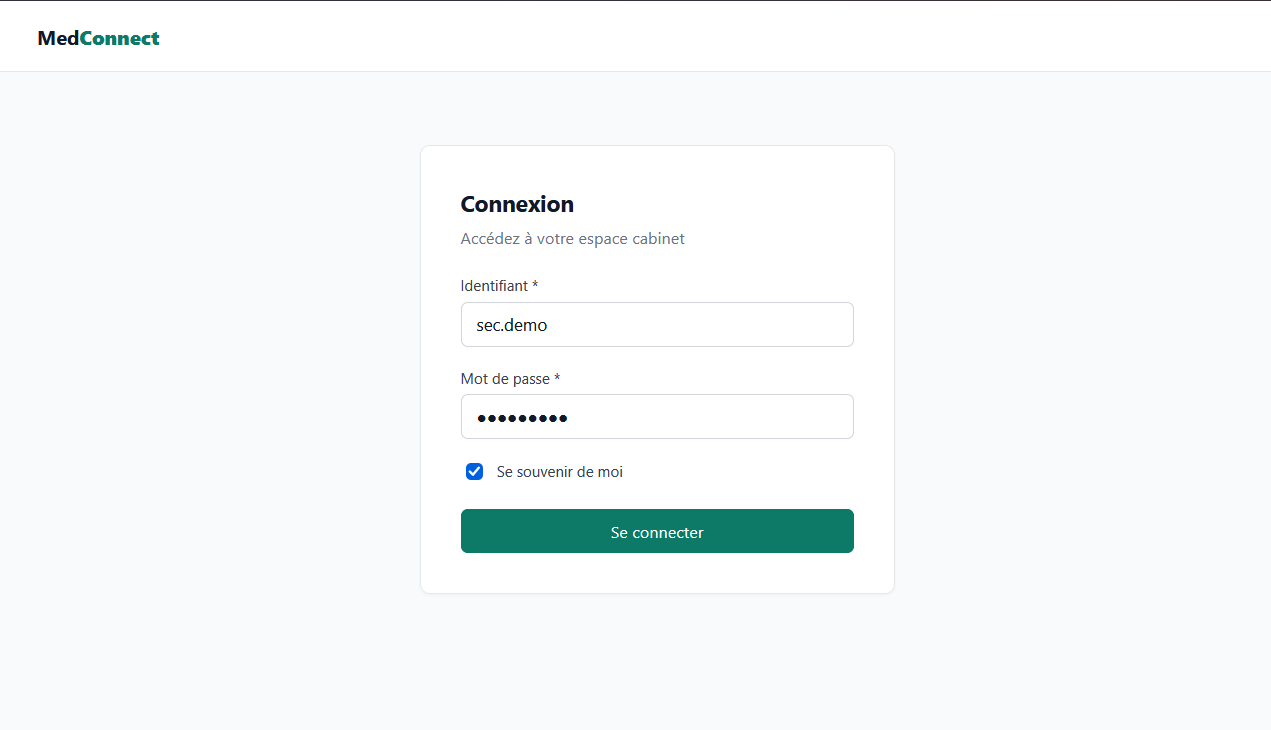
\includegraphics[width=0.75\textwidth]{login.png}
  \caption{Page de connexion MedConnect – authentification JWT}
  \label{fig:login}
\end{figure}

\section{Gestion des patients}

\begin{figure}[H]
  \centering
  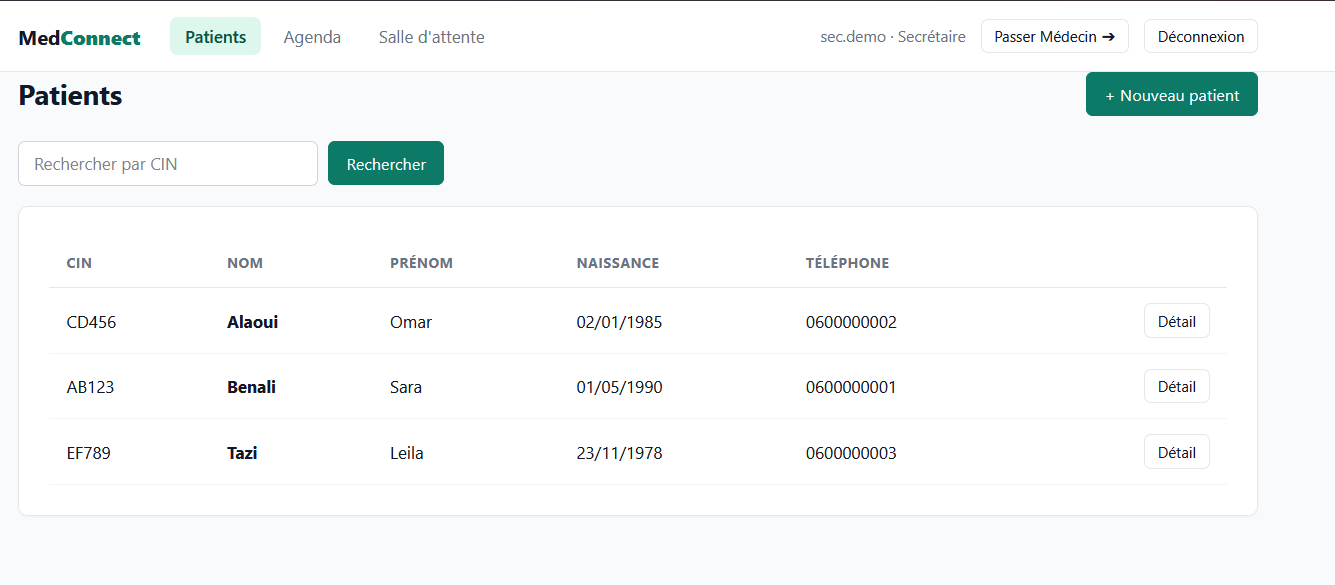
\includegraphics[width=0.85\textwidth]{patient1.png}
  \caption{Liste des patients avec recherche par CIN ou nom}
  \label{fig:patients-list}
\end{figure}

\begin{figure}[H]
  \centering
  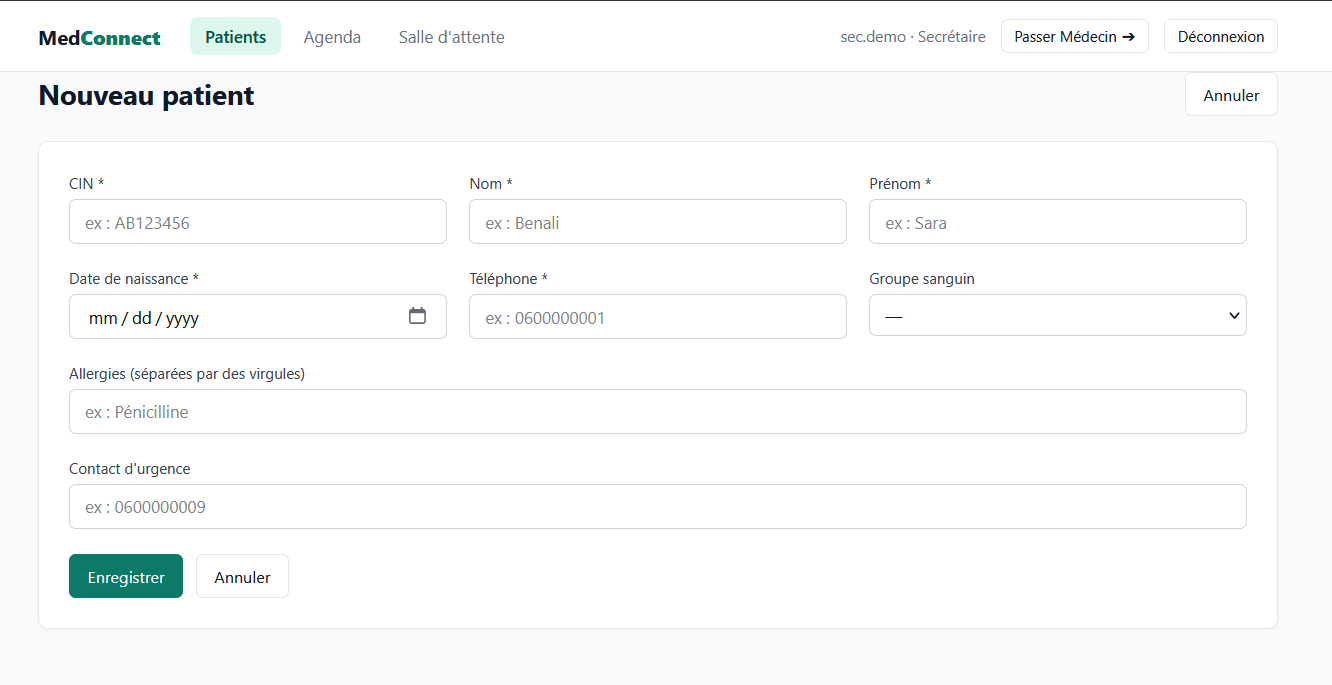
\includegraphics[width=0.85\textwidth]{patient2.png}
  \caption{Formulaire d'ajout d'un nouveau patient}
  \label{fig:patients-add}
\end{figure}

\begin{figure}[H]
  \centering
  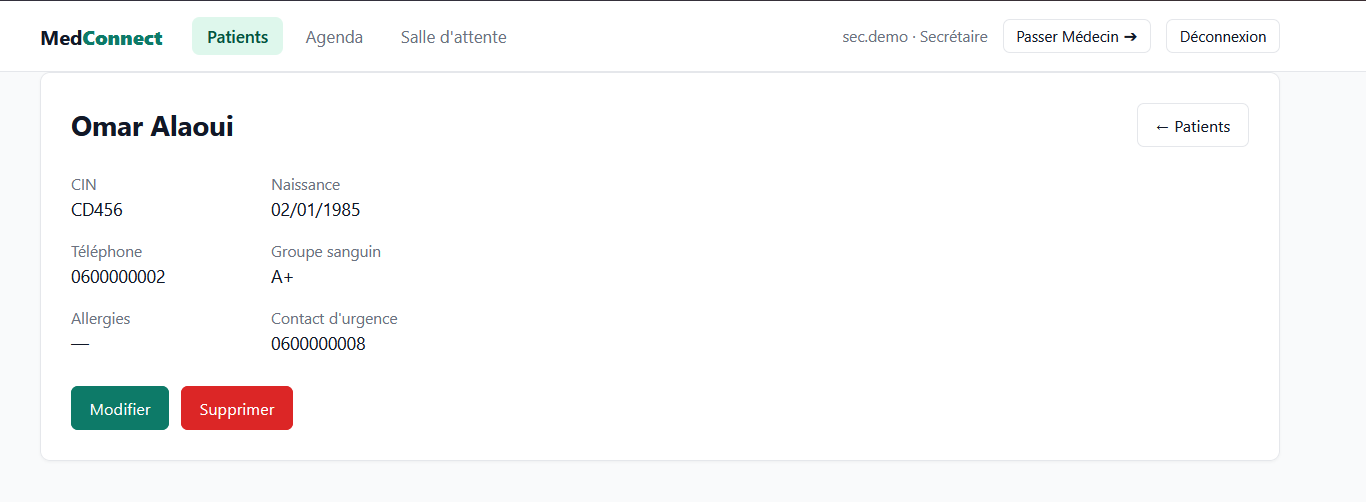
\includegraphics[width=0.85\textwidth]{patient3.png}
  \caption{Détail et modification des informations d'un patient}
  \label{fig:patients-detail}
\end{figure}

\section{Gestion de l'agenda et des rendez-vous}

\begin{figure}[H]
  \centering
  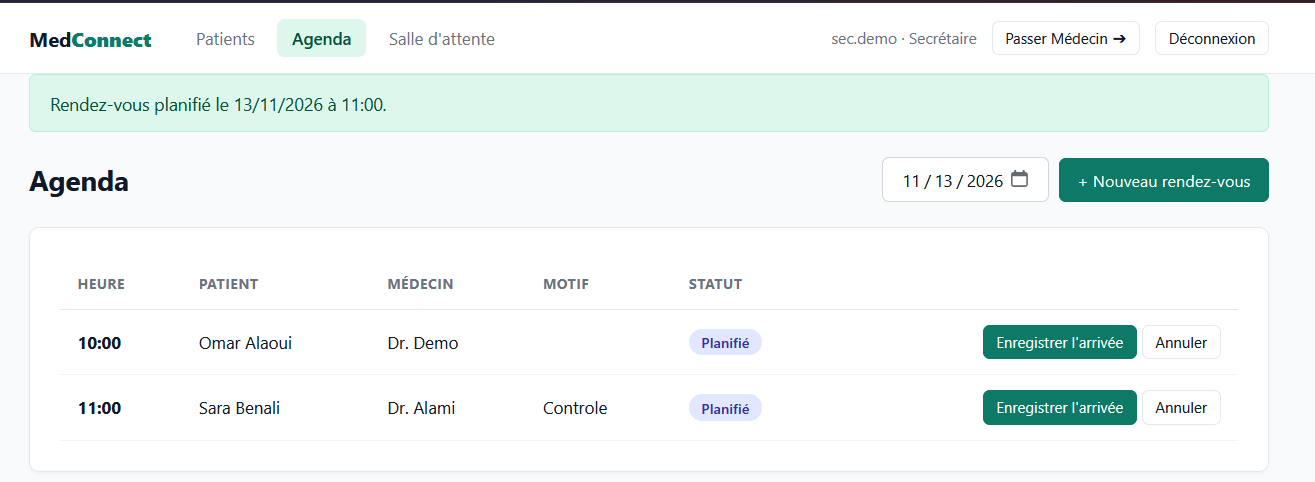
\includegraphics[width=0.85\textwidth]{Agenda1.png}
  \caption{Vue principale de l'agenda – liste des rendez-vous planifiés}
  \label{fig:agenda-list}
\end{figure}

\begin{figure}[H]
  \centering
  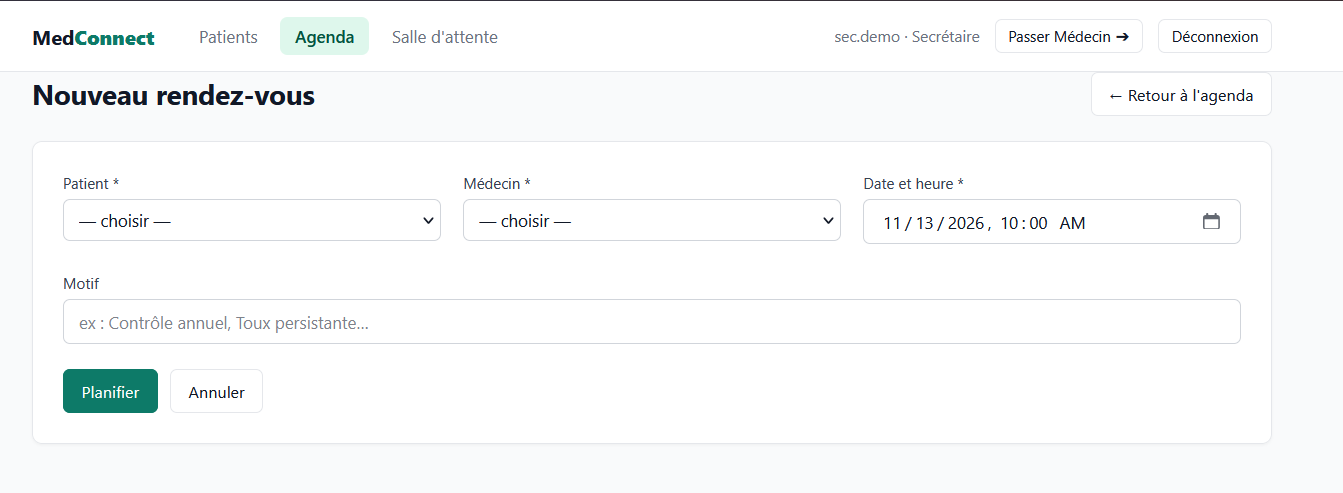
\includegraphics[width=0.85\textwidth]{Agenda2.png}
  \caption{Formulaire de prise de rendez-vous avec sélection du médecin}
  \label{fig:agenda-create}
\end{figure}

\begin{figure}[H]
  \centering
  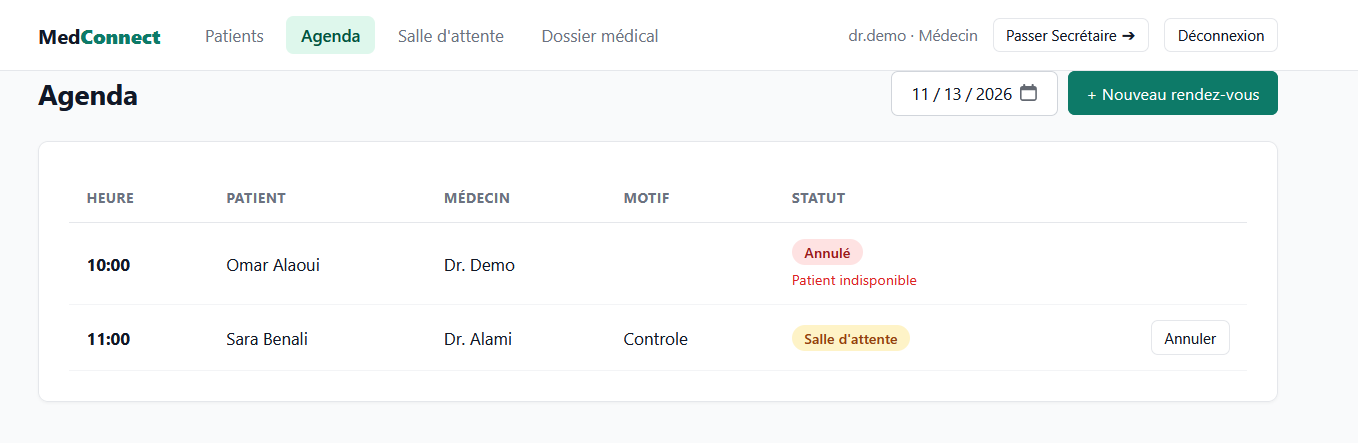
\includegraphics[width=0.85\textwidth]{agenda3.png}
  \caption{Avancement du statut d'un rendez-vous (Planifié → Salle d'attente)}
  \label{fig:agenda-advance}
\end{figure}

\begin{figure}[H]
  \centering
  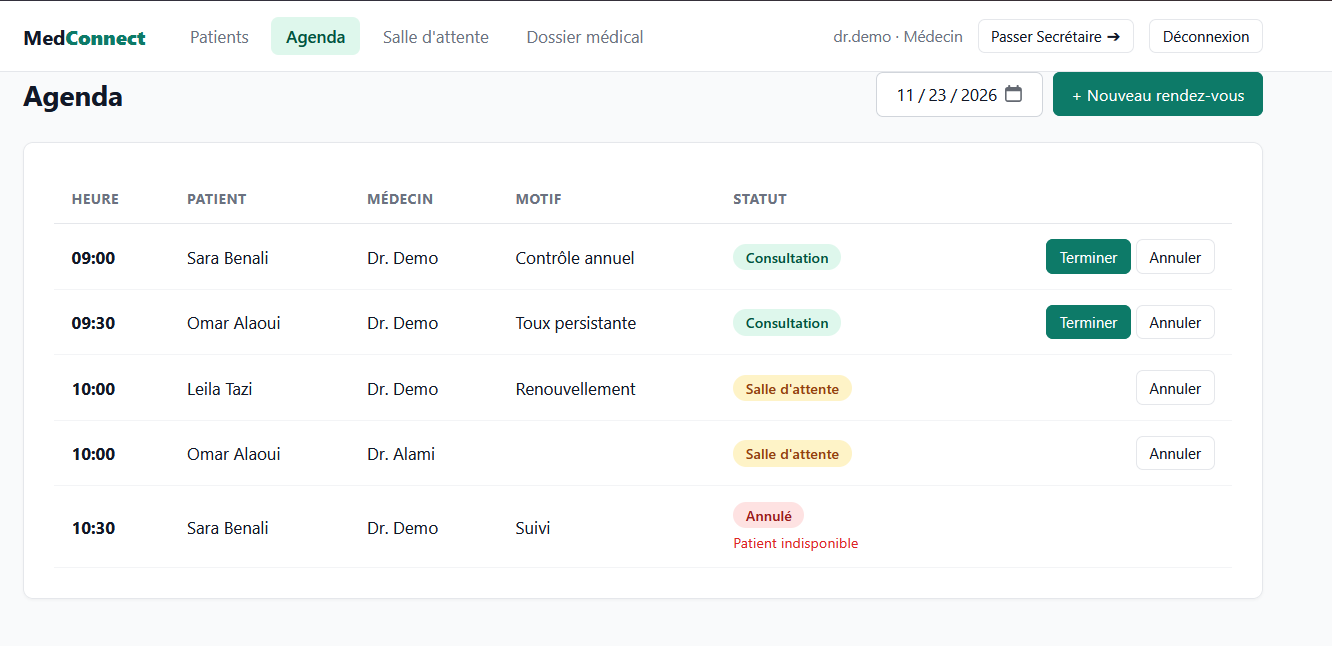
\includegraphics[width=0.85\textwidth]{agenda4.png}
  \caption{Vue détaillée de l'agenda avec filtrage et statuts en temps réel}
  \label{fig:agenda-view4}
\end{figure}

\begin{figure}[H]
  \centering
  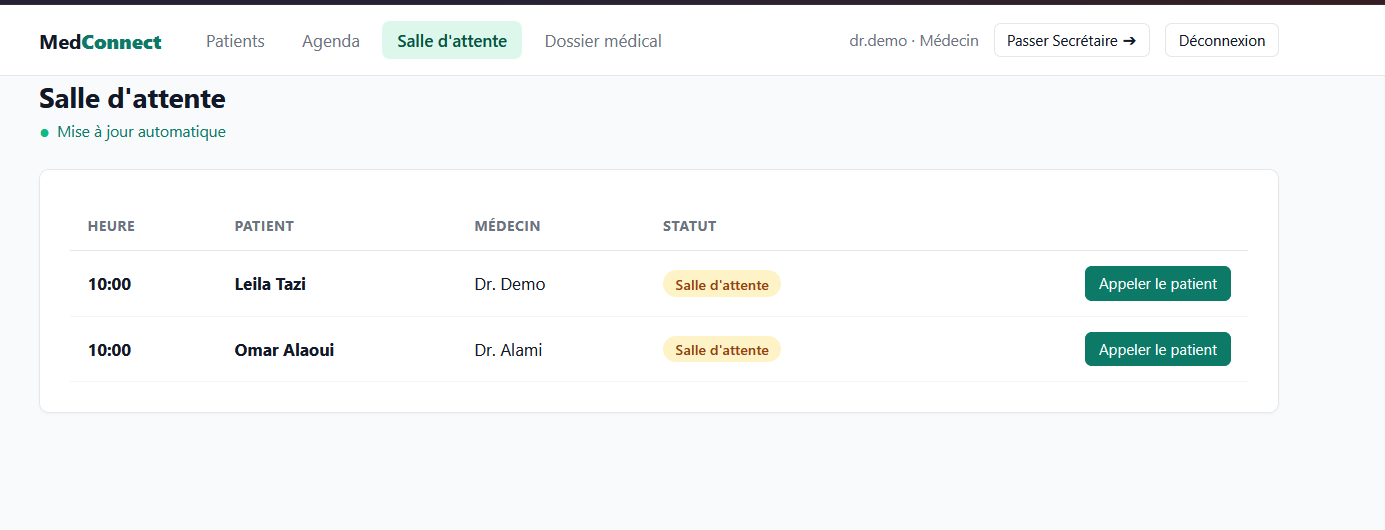
\includegraphics[width=0.85\textwidth]{salle attente.png}
  \caption{Salle d'attente – gestion de la file d'attente et appel en consultation}
  \label{fig:salle-attente-dedicated}
\end{figure}

\begin{figure}[H]
  \centering
  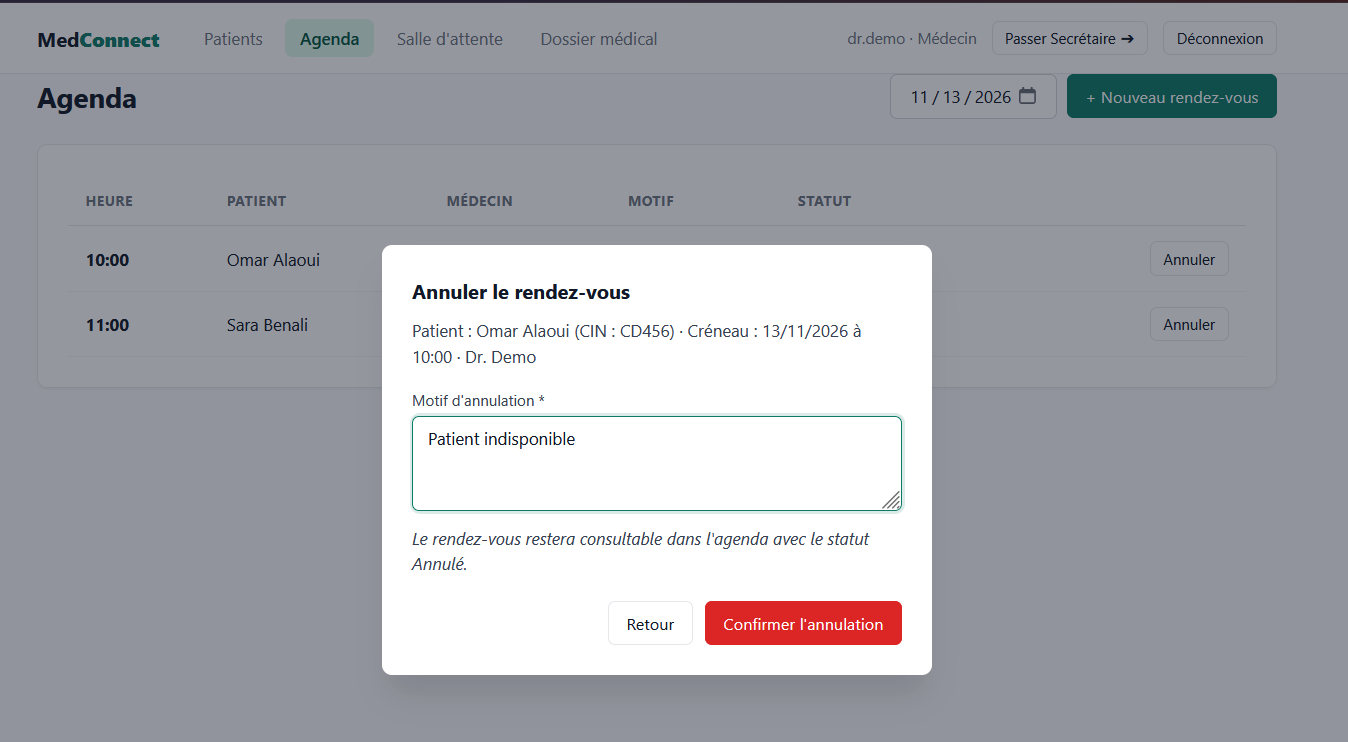
\includegraphics[width=0.85\textwidth]{agenda_anulation.png}
  \caption{Confirmation d'annulation d'un rendez-vous}
  \label{fig:agenda-cancel}
\end{figure}

\section{Dossier médical}

\begin{figure}[H]
  \centering
  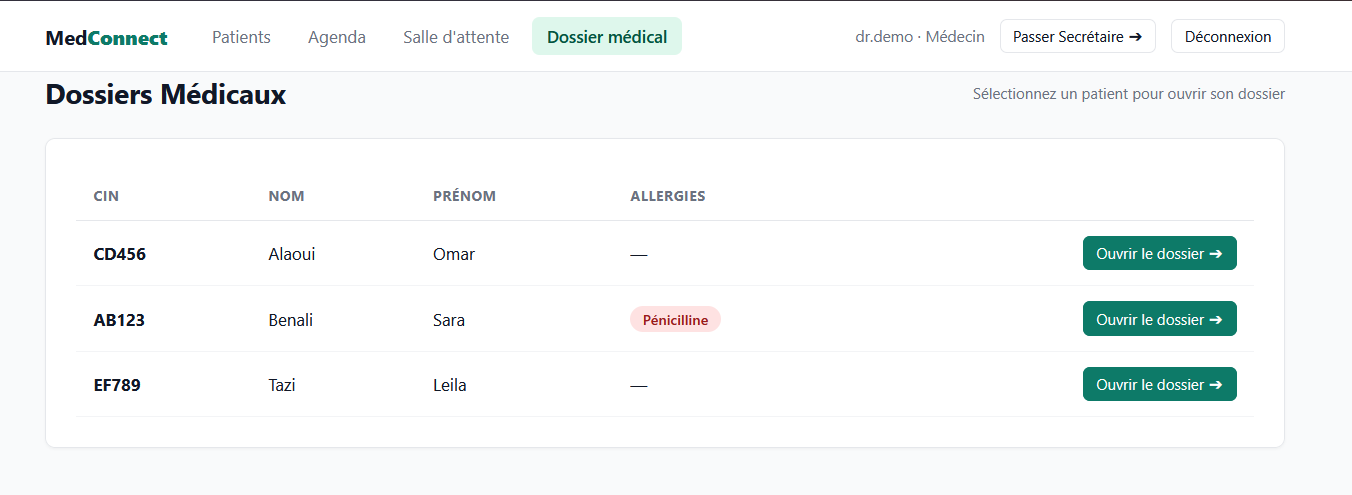
\includegraphics[width=0.85\textwidth]{dossier medical.png}
  \caption{Dossier médical électronique – historique des consultations}
  \label{fig:dossier-list}
\end{figure}

\begin{figure}[H]
  \centering
  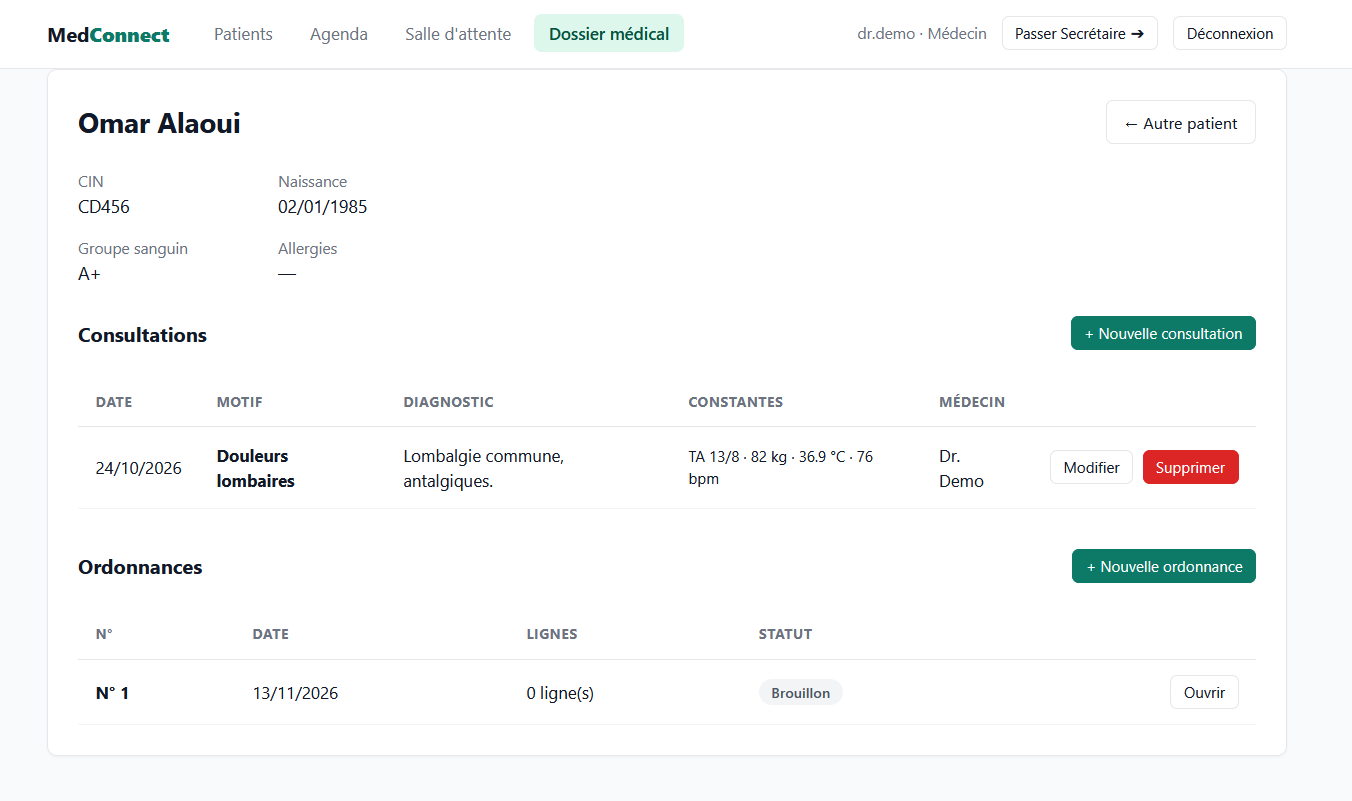
\includegraphics[width=0.85\textwidth]{dossier medical2.png}
  \caption{Formulaire de création d'une nouvelle consultation}
  \label{fig:dossier-create}
\end{figure}

\section{Ordonnances}

\begin{figure}[H]
  \centering
  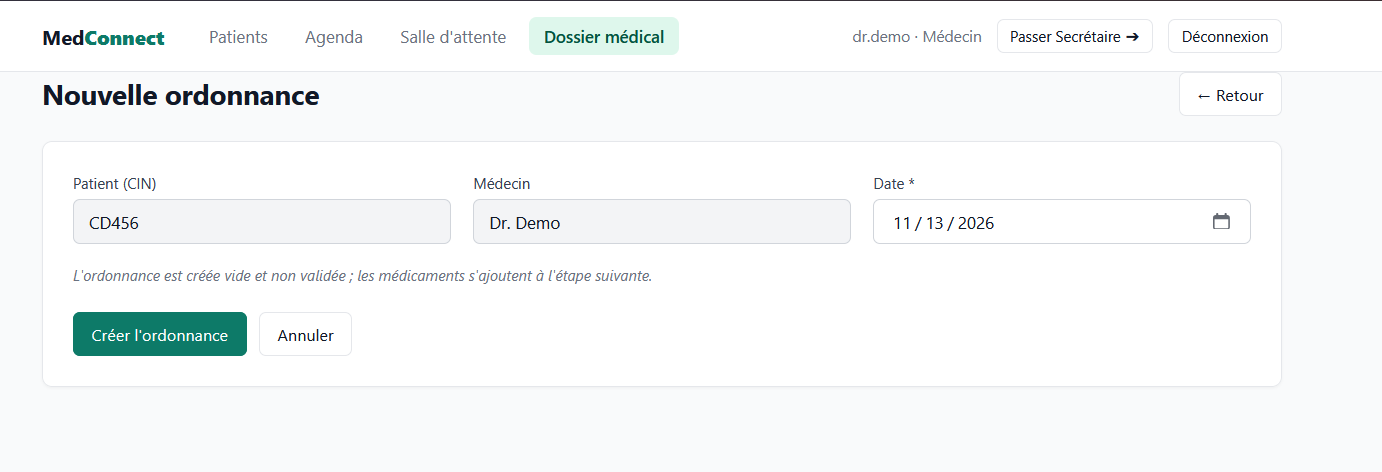
\includegraphics[width=0.85\textwidth]{ordonnace1.png}
  \caption{Création d'une ordonnance et ajout de médicaments}
  \label{fig:ordonnance-create}
\end{figure}

\begin{figure}[H]
  \centering
  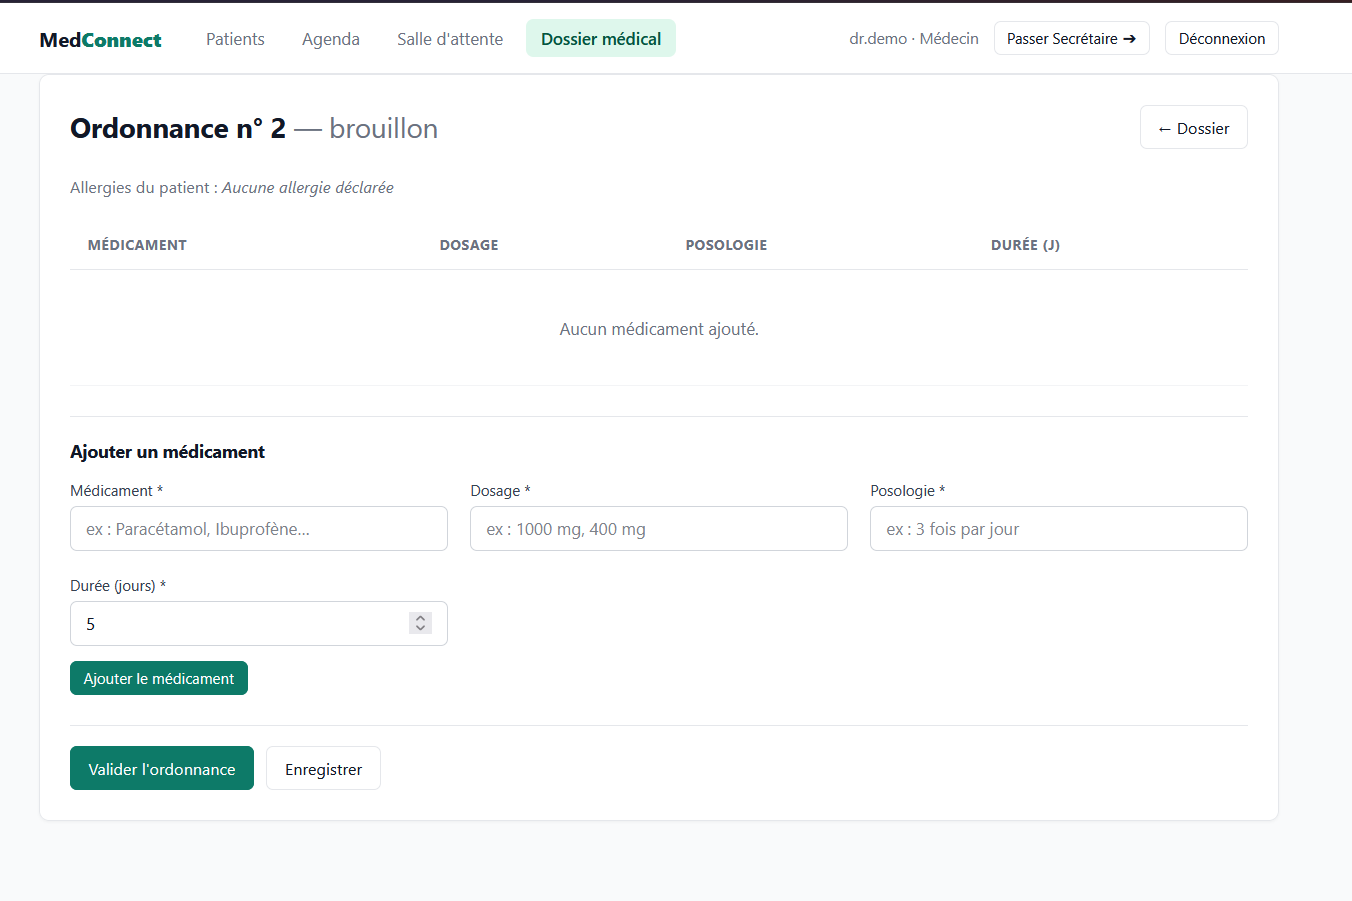
\includegraphics[width=0.85\textwidth]{ordonnace2.png}
  \caption{Validation de l'ordonnance – état immuable après validation}
  \label{fig:ordonnance-validate}
\end{figure}

% ══════════════════════════════════════════════════════
%  SECTION 9 : TESTS ET ASSURANCE QUALITÉ
% ══════════════════════════════════════════════════════
\chapter{Campagne de Tests et Assurance Qualité}

\section{Stratégie de test}

La stratégie de test de MedConnect repose sur deux niveaux complémentaires :

\begin{itemize}[leftmargin=*]
  \item \textbf{Tests unitaires (Pytest)} : 23 tests couvrant la logique métier indépendamment du framework Django (sérialisation, règles métier, algorithme d'allergie).
  \item \textbf{Tests d'intégration API (Django TestCase)} : 45 tests couvrant l'intégralité des endpoints REST avec simulation de requêtes HTTP authentifiées, vérification des codes de réponse et validation des payloads JSON.
\end{itemize}

\section{Tests unitaires Pytest}

\begin{table}[H]
\centering
\caption{Résultats des tests unitaires Pytest (23 tests)}
\renewcommand{\arraystretch}{1.4}
\begin{tabular}{|p{5cm}|c|c|c|}
  \hline
  \rowcolor{medaccent}
  \textbf{Fichier de test} & \textbf{Tests} & \textbf{Réussis} & \textbf{Statut} \\
  \hline
  \texttt{test\_patients.py} & 6 & 6 & \textcolor{medgreen}{\textbf{PASS}} \\
  \hline
  \texttt{test\_agenda.py} & 7 & 7 & \textcolor{medgreen}{\textbf{PASS}} \\
  \hline
  \texttt{test\_dossier.py} & 5 & 5 & \textcolor{medgreen}{\textbf{PASS}} \\
  \hline
  \texttt{test\_ordonnances.py} & 5 & 5 & \textcolor{medgreen}{\textbf{PASS}} \\
  \hline
  \rowcolor{medgreen!20}
  \textbf{Total} & \textbf{23} & \textbf{23} & \textcolor{medgreen}{\textbf{100\% PASS}} \\
  \hline
\end{tabular}
\end{table}

\section{Tests d'intégration API Django REST}

\begin{table}[H]
\centering
\caption{Résultats des tests API Django (45 tests)}
\renewcommand{\arraystretch}{1.4}
\begin{tabular}{|p{5cm}|c|c|c|}
  \hline
  \rowcolor{medaccent}
  \textbf{Module} & \textbf{Tests} & \textbf{Réussis} & \textbf{Statut} \\
  \hline
  \texttt{patients\_api} & 5 & 5 & \textcolor{medgreen}{\textbf{PASS}} \\
  \hline
  \texttt{agenda\_api} & 16 & 16 & \textcolor{medgreen}{\textbf{PASS}} \\
  \hline
  \texttt{dossier\_medical\_api} & 21 & 21 & \textcolor{medgreen}{\textbf{PASS}} \\
  \hline
  \texttt{ordonnances\_api} & 3 & 3 & \textcolor{medgreen}{\textbf{PASS}} \\
  \hline
  \rowcolor{medgreen!20}
  \textbf{Total} & \textbf{45} & \textbf{45} & \textcolor{medgreen}{\textbf{100\% PASS}} \\
  \hline
\end{tabular}
\end{table}

\textbf{Récapitulatif global :} \textbf{68/68 tests réussis} (100\% de taux de succès).

\section{Résultats visuels}

\begin{figure}[H]
  \centering
  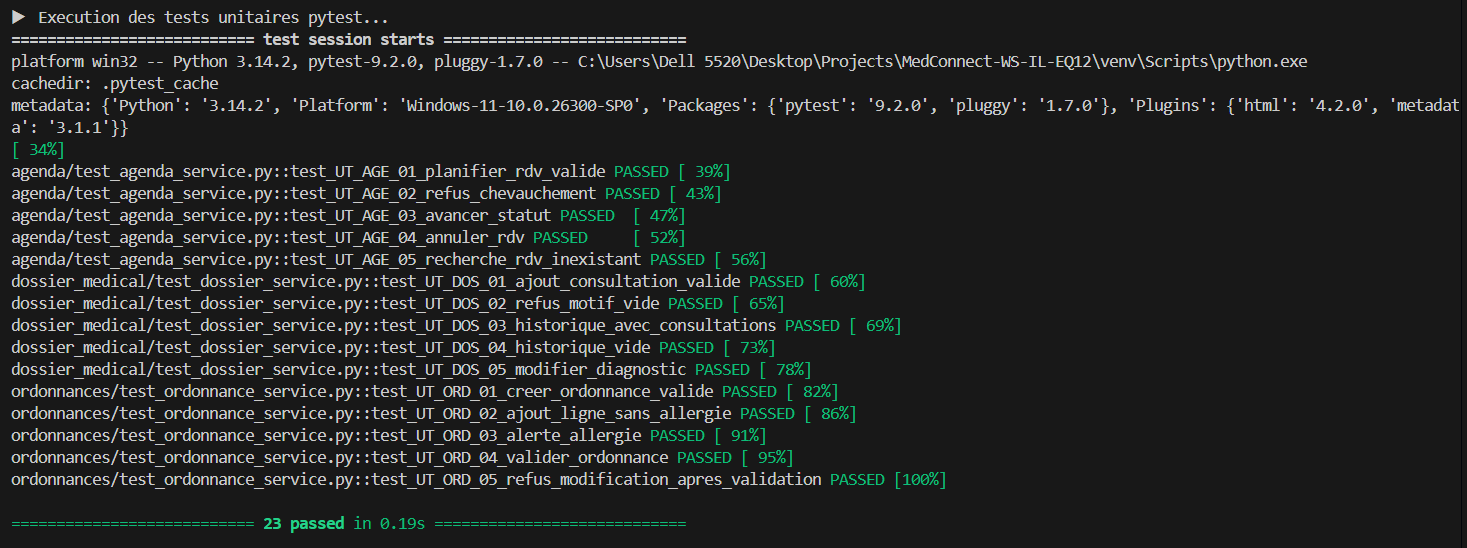
\includegraphics[width=0.9\textwidth]{pytest terminal.png}
  \caption{Résultats Pytest en sortie terminal – 23/23 tests passants}
  \label{fig:pytest-terminal}
\end{figure}

\begin{figure}[H]
  \centering
  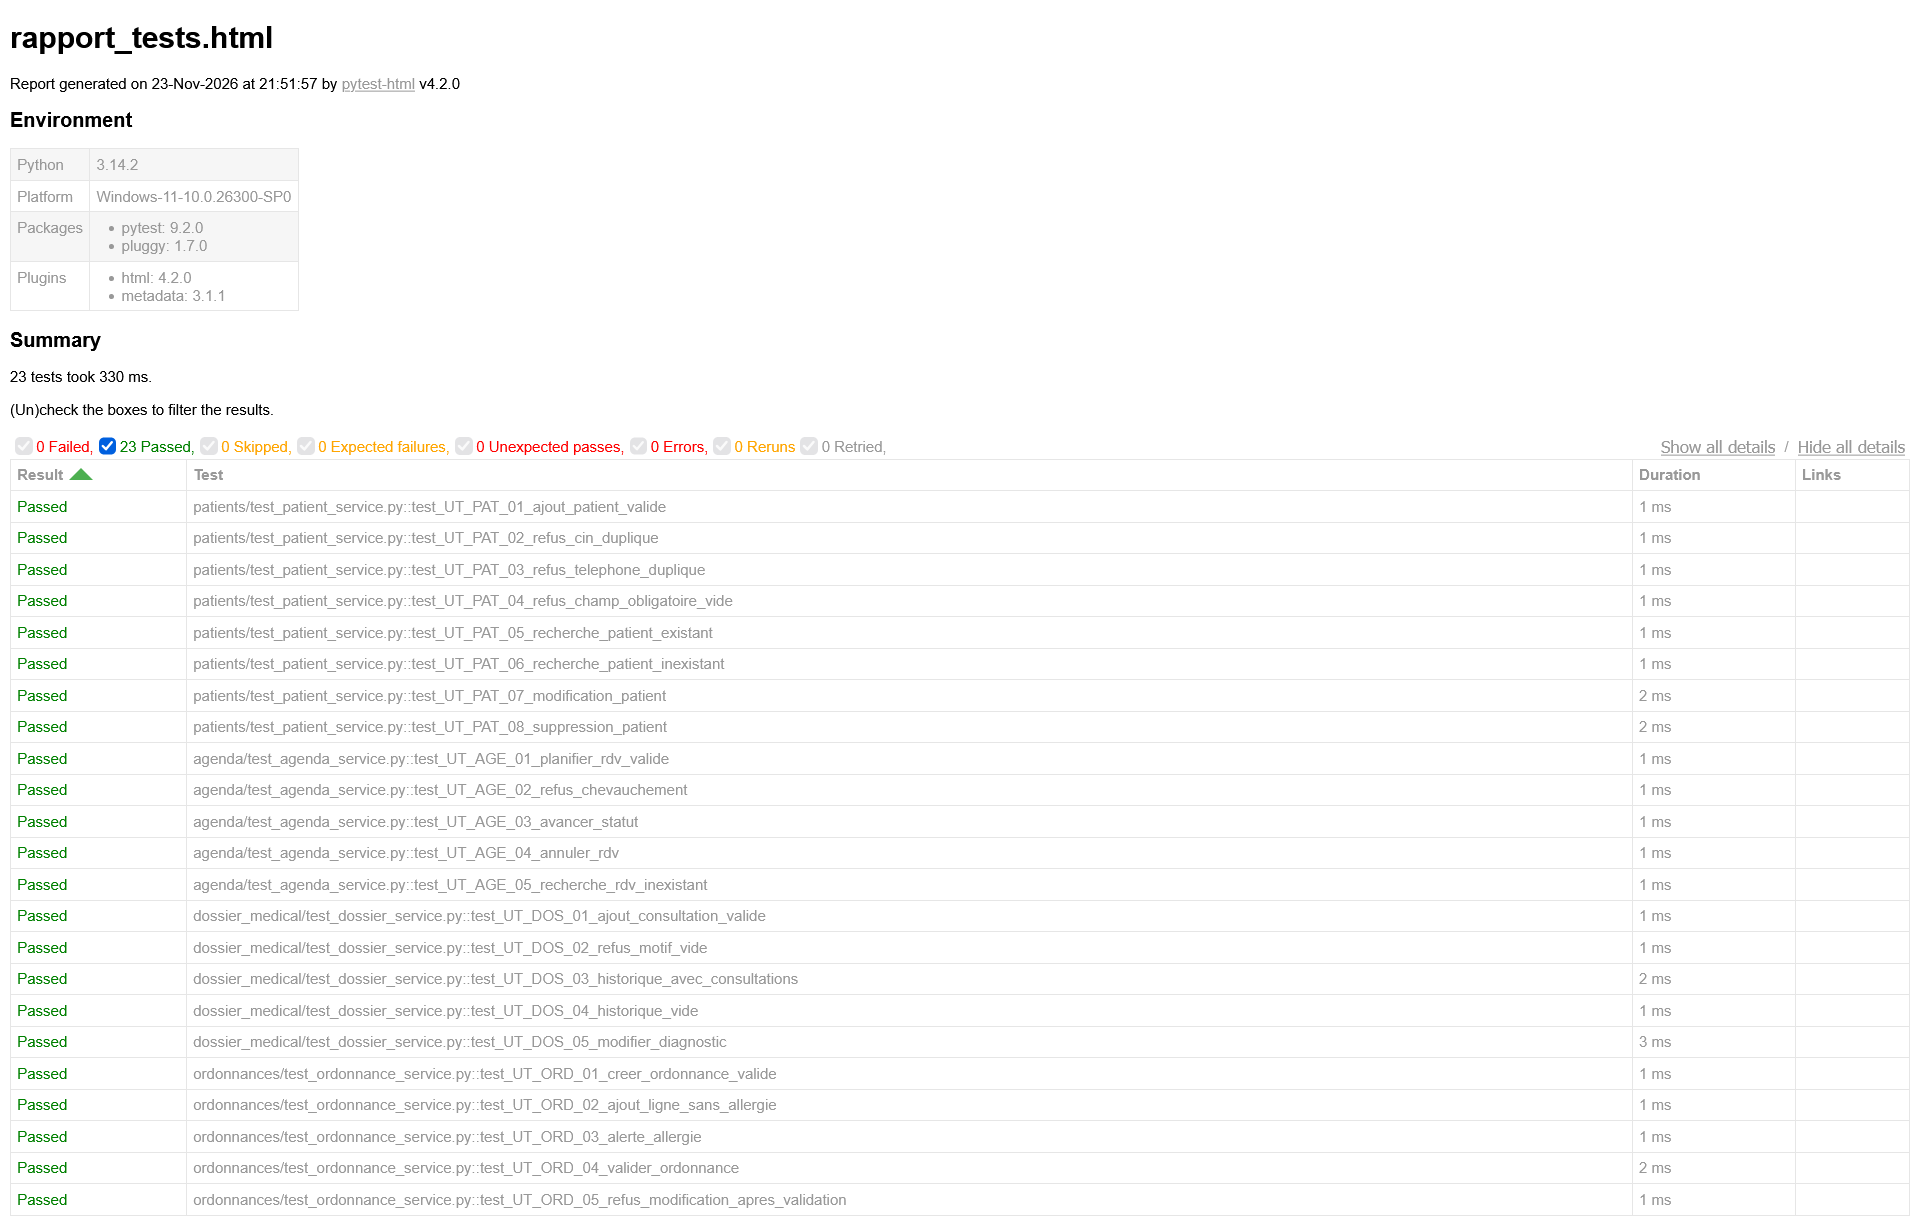
\includegraphics[width=0.9\textwidth]{pytest htmlreport.png}
  \caption{Rapport HTML pytest-html – détail des 23 tests unitaires}
  \label{fig:pytest-html}
\end{figure}

\section{Détail des scénarios de test clés}

\begin{itemize}[leftmargin=*]
  \item \textbf{Création patient avec CIN en doublon} : retourne \texttt{HTTP 400} avec message d'erreur explicite.
  \item \textbf{Avancement de statut hors séquence} : tentative de passer de Planifié à Terminé directement → \texttt{HTTP 400}.
  \item \textbf{Annulation d'un RDV déjà Terminé} : retourne \texttt{HTTP 400}.
  \item \textbf{Ajout de ligne sur ordonnance validée} : retourne \texttt{HTTP 400} (immuabilité).
  \item \textbf{Détection d'allergie} : médicament correspondant à une allergie déclarée → avertissement dans la réponse.
  \item \textbf{Accès secrétaire aux dossiers médicaux} : retourne \texttt{HTTP 403} (RBAC).
  \item \textbf{Requête sans token JWT} : retourne \texttt{HTTP 401} sur tout endpoint protégé.
  \item \textbf{Refresh token expiré} : retourne \texttt{HTTP 401} avec message de réauthentification.
\end{itemize}

% ══════════════════════════════════════════════════════
%  SECTION 10 : DÉPLOIEMENT ET EXÉCUTION
% ══════════════════════════════════════════════════════
\chapter{Déploiement et Exécution}

\section{Prérequis}

\begin{itemize}[leftmargin=*]
  \item Python 3.11+ (testé sur Python 3.14.2)
  \item Git
  \item Navigateur web moderne (Chrome, Firefox, Edge)
  \item Connexion Internet pour l'installation des dépendances
\end{itemize}

\section{Installation et lancement}

\begin{lstlisting}[language=bash, caption={Procédure d'installation complète}]
# 1. Cloner le dépôt
git clone https://github.com/AllabouchAnas/MedConnect-WS-IL-EQ12.git
cd MedConnect-WS-IL-EQ12/backend

# 2. Créer et activer l'environnement virtuel
python -m venv venv
# Windows
venv\Scripts\activate
# Linux / macOS
source venv/bin/activate

# 3. Installer les dépendances
pip install -r requirements.txt

# 4. Appliquer les migrations
python manage.py migrate

# 5. Peupler la base de données de démo
python seed_demo.py

# 6. Lancer le serveur de développement
python manage.py runserver
\end{lstlisting}

\section{Déploiement conteneurisé avec Docker et Docker Compose}

Afin de garantir la portabilité, l'isolation des environnements et une mise en production simplifiée, MedConnect intègre une infrastructure de conteneurisation complète reposant sur \textbf{Docker} et \textbf{Docker Compose}, couplant l'application Django avec un serveur de base de données relationnelle \textbf{PostgreSQL 16}.

\subsection{Architecture des conteneurs}

Le déploiement s'articule autour de deux services interconnectés via un réseau virtuel Docker isolé :

\begin{itemize}[leftmargin=*]
  \item \textbf{Service \texttt{db}} : Conteneur basé sur l'image officielle \texttt{postgres:16-alpine}. Les données sont persistées sur le volume managé \texttt{pgdata}. Un test de santé (\textit{healthcheck}) via \texttt{pg\_isready} valide la disponibilité du moteur avant le démarrage du backend.
  \item \textbf{Service \texttt{web}} : Conteneur applicatif basé sur \texttt{python:3.12-slim}. L'application est servie par le serveur WSGI de production \textbf{Gunicorn} avec 3 workers sur le port \texttt{8000}. La distribution des fichiers statiques est prise en charge par \textbf{WhiteNoise}. L'exécution est sécurisée sous un utilisateur dédié non-root (\texttt{app:app}, UID 1000).
\end{itemize}

\subsection{Script d'entrée automatique (\texttt{docker-entrypoint.sh})}

Au démarrage du conteneur \texttt{web}, le point d'entrée exécute automatiquement et séquentiellement :
\begin{enumerate}[leftmargin=*]
  \item L'application des migrations de schéma (\texttt{python manage.py migrate}).
  \item Le rassemblement des fichiers statiques frontend (\texttt{python manage.py collectstatic --noinput}).
  \item Le peuplement conditionnel des comptes et données de démo (\texttt{seed\_demo.py} si \texttt{SEED\_DEMO=1}).
  \item Le lancement du serveur Gunicorn en écoute sur \texttt{0.0.0.0:8000}.
\end{enumerate}

\subsection{Variables d'environnement}

\begin{table}[H]
\centering
\caption{Variables d'environnement supportées par la pile Docker}
\renewcommand{\arraystretch}{1.4}
\begin{tabular}{|p{4.5cm}|p{3.5cm}|p{6cm}|}
  \hline
  \rowcolor{medaccent}
  \textbf{Variable} & \textbf{Valeur par défaut} & \textbf{Description} \\
  \hline
  \texttt{DJANGO\_SECRET\_KEY} & clé générée dev & Clé cryptographique Django (à modifier en prod) \\
  \hline
  \texttt{DB\_PASSWORD} & \texttt{medconnect-dev} & Mot de passe de l'utilisateur PostgreSQL \\
  \hline
  \texttt{DJANGO\_ALLOWED\_HOSTS} & \texttt{localhost,127.0.0.1} & Noms d'hôtes HTTP autorisés \\
  \hline
  \texttt{SEED\_DEMO} & \texttt{1} & Activer (1) ou désactiver (0) l'injection de démo \\
  \hline
  \texttt{DB\_ENGINE} & \texttt{postgres} & Sélecteur du moteur de base de données \\
  \hline
  \texttt{DB\_HOST} & \texttt{db} & Hôte réseau du conteneur PostgreSQL \\
  \hline
\end{tabular}
\end{table}

\subsection{Commandes d'exploitation Docker}

\begin{lstlisting}[language=bash, caption={Commandes usuelles de gestion Docker}]
# Lancer la pile complete (build + execution)
docker compose up --build

# Lancer en arriere-plan (mode detache)
docker compose up -d --build

# Consulter les journaux applicatifs en direct
docker compose logs -f web

# Executer la suite de tests Django dans le conteneur
docker compose run --rm -e SEED_DEMO=0 web python manage.py test

# Arreter les conteneurs (donnees conservees)
docker compose down

# Arret complet et purge de la base de donnees (volume supprime)
docker compose down -v
\end{lstlisting}

\section{Exécution des tests}

\begin{lstlisting}[language=bash, caption={Lancement de la suite de tests complète}]
# Tests unitaires Pytest (23 tests)
cd backend
pytest tests/ -v --html=pytest-report.html

# Tests API Django (45 tests)
python manage.py test patients_api agenda_api dossier_medical_api ordonnances_api -v
\end{lstlisting}

\section{Comptes de démonstration}

\begin{table}[H]
\centering
\caption{Comptes de démonstration créés par \texttt{seed\_demo.py}}
\renewcommand{\arraystretch}{1.4}
\begin{tabular}{|p{3.5cm}|p{3.5cm}|p{3.5cm}|p{3cm}|}
  \hline
  \rowcolor{medaccent}
  \textbf{Identifiant} & \textbf{Mot de passe} & \textbf{Rôle} & \textbf{Groupe Django} \\
  \hline
  \texttt{dr.demo} & \texttt{Demo@1234} & Médecin & Medecin \\
  \hline
  \texttt{sec.demo} & \texttt{Demo@1234} & Secrétaire & Secretaire \\
  \hline
\end{tabular}
\end{table}

% ══════════════════════════════════════════════════════
%  SECTION 11 : ORGANISATION DU TRAVAIL
% ══════════════════════════════════════════════════════
\chapter{Organisation du Travail}

\section{Répartition des tâches}

\begin{table}[H]
\centering
\caption{Répartition des responsabilités par membre}
\renewcommand{\arraystretch}{1.4}
\begin{tabularx}{\textwidth}{|p{3.5cm}|p{3cm}|X|}
  \hline
  \rowcolor{medaccent}
  \textbf{Membre} & \textbf{Rôle} & \textbf{Contributions} \\
  \hline
  Allabouch Anass & Chef de Projet & Architecture globale, \texttt{patients\_api}, configuration Django/JWT, script \texttt{seed\_demo.py}, intégration et rapport \\
  \hline
  Ahmed Lahmaine & Product Owner / BA & \texttt{agenda\_api}, gestion des statuts RDV, salle d'attente, liste des médecins, feature branch \\
  \hline
  Achraf Ait Damnat & Lead Tech / Architecte & \texttt{dossier\_medical\_api}, modèle de consultation, paramètres cliniques, intégration frontend \\
  \hline
  Abdellah Rahel & QA / Conformité & \texttt{ordonnances\_api}, algorithme d'allergie, règle d'immuabilité, campagne de tests \\
  \hline
\end{tabularx}
\end{table}

\section{Workflow Git}

L'équipe a adopté un workflow Git structuré inspiré de Gitflow :

\begin{itemize}[leftmargin=*]
  \item \textbf{\texttt{main}} : Branche de production – contient le code stable et intégré.
  \item \textbf{\texttt{develop}} : Branche d'intégration – fusion de toutes les features avant promotion vers main.
  \item \textbf{\texttt{feature/agenda-api}} : Développement de l'agenda (Ahmed Lahmaine) – mergée via Pull Request.
  \item \textbf{\texttt{feature/dossier-medical-api}} : Développement du dossier médical (Achraf Ait Damnat).
  \item \textbf{\texttt{feature/ordonnances-api}} : Développement des ordonnances (Abdellah Rahel).
\end{itemize}

Chaque Pull Request requiert une revue de code et la réussite des tests avant fusion.

\section{Instructions de fusion pour les membres de l'équipe}

Les instructions détaillées pour que chaque membre pousse son module vers \texttt{main} se trouvent dans \texttt{README.md} du dépôt (branche \texttt{develop}). La procédure type est :

\begin{lstlisting}[language=bash, caption={Procédure de contribution individuelle}]
# 1. Se positionner sur sa feature branch
git checkout feature/[mon-module]-api

# 2. Synchroniser avec develop
git fetch origin
git rebase origin/develop

# 3. Ouvrir une Pull Request sur GitHub : feature/* -> develop
# 4. Après validation de l'équipe : merge dans develop
# 5. Chef de projet : merge develop -> main après validation globale
\end{lstlisting}

\section{Difficultés rencontrées}

\begin{itemize}[leftmargin=*]
  \item \textbf{Incompatibilité PowerShell} : L'opérateur \texttt{\&\&} n'est pas supporté nativement dans PowerShell Windows, ce qui a nécessité l'utilisation du script \texttt{exe.py} comme alternative cross-platform.
  \item \textbf{Avertissement clé JWT} : Django 6.0 avec SimpleJWT génère un avertissement si la \texttt{SECRET\_KEY} est trop courte – résolu en générant une clé de 50 caractères.
  \item \textbf{Peuplement BDD} : Le script \texttt{seed\_demo.py} doit gérer le cas où les données de démo existent déjà (utilisation de \texttt{get\_or\_create}).
  \item \textbf{Noms de fichiers avec espaces} : Certains screenshots contiennent des espaces dans leur nom (\texttt{dossier medical.png}, \texttt{salle attente.png}) – gérés directement dans le \texttt{.tex} sans renommage.
  \item \textbf{Coordination multi-branches} : Synchronisation des quatre feature branches sans conflits a nécessité une discipline stricte dans les périmètres de modèles.
\end{itemize}

% ══════════════════════════════════════════════════════
%  SECTION 12 : BILAN QUALITÉ
% ══════════════════════════════════════════════════════
\chapter{Bilan Qualité}

\section{Couverture des tests}

\begin{table}[H]
\centering
\caption{Bilan de la couverture de tests par module}
\renewcommand{\arraystretch}{1.4}
\begin{tabular}{|p{4cm}|c|c|c|c|}
  \hline
  \rowcolor{medaccent}
  \textbf{Module} & \textbf{Tests U.} & \textbf{Tests API} & \textbf{Total} & \textbf{Taux} \\
  \hline
  \texttt{patients\_api} & 6 & 5 & 11 & \textcolor{medgreen}{100\%} \\
  \hline
  \texttt{agenda\_api} & 7 & 16 & 23 & \textcolor{medgreen}{100\%} \\
  \hline
  \texttt{dossier\_medical\_api} & 5 & 21 & 26 & \textcolor{medgreen}{100\%} \\
  \hline
  \texttt{ordonnances\_api} & 5 & 3 & 8 & \textcolor{medgreen}{100\%} \\
  \hline
  \rowcolor{medgreen!20}
  \textbf{Total} & \textbf{23} & \textbf{45} & \textbf{68} & \textcolor{medgreen}{\textbf{100\%}} \\
  \hline
\end{tabular}
\end{table}

\section{Qualité du code}

\begin{itemize}[leftmargin=*]
  \item \textbf{Conformité REST} : Codes HTTP sémantiquement corrects (201 pour création, 204 pour suppression, 400 pour erreur client, 401/403 pour sécurité).
  \item \textbf{Séparation des responsabilités} : Chaque module respecte la séparation \texttt{models.py / serializers.py / views.py / urls.py}.
  \item \textbf{Pas de logique dans les vues} : Les règles métier (détection allergie, immuabilité, flux de statut) sont encapsulées dans les sérialiseurs ou des méthodes de modèle.
  \item \textbf{Pas de code dupliqué} : Les permissions \texttt{HasCabinetRole} et \texttt{IsMedecin} sont définies une seule fois dans un module \texttt{permissions.py} partagé.
  \item \textbf{Nommage cohérent} : Conventions snake\_case Python respectées, noms de variables et commentaires en français.
\end{itemize}

% ══════════════════════════════════════════════════════
%  SECTION 13 : LIMITES ET PERSPECTIVES
% ══════════════════════════════════════════════════════
\chapter{Limites et Perspectives}

\section{Limites fonctionnelles}

\begin{itemize}[leftmargin=*]
  \item \textbf{Interface multi-médecins limitée} : Le filtre par médecin dans la vue agenda est opérationnel côté API mais l'interface frontend ne propose pas encore de sélecteur de médecin dans la vue calendrier.
  \item \textbf{Pas de notifications} : Aucune notification email ou SMS n'est implémentée pour rappeler les rendez-vous aux patients.
  \item \textbf{Pas de gestion documentaire} : Les ordonnances sont stockées en JSON uniquement – pas de génération PDF à ce stade.
  \item \textbf{Pas de pagination avancée} : La pagination est implémentée mais sans navigation par curseur pour les très grandes listes.
  \item \textbf{Mono-cabinet} : L'application gère un seul cabinet – pas de support multi-sites.
\end{itemize}

\section{Dettes techniques}

\begin{itemize}[leftmargin=*]
  \item \textbf{Absence de CI/CD} : Pas de pipeline d'intégration continue automatisé (GitHub Actions ou GitLab CI).
  \item \textbf{Pas de documentation Swagger/OpenAPI} : L'API n'expose pas encore d'interface Swagger interactive (drf-spectacular ou drf-yasg).
  \item \textbf{\texttt{db.sqlite3} hors Git} : Le fichier SQLite local est exclu du versionning (\texttt{.gitignore}) – le script \texttt{seed\_demo.py} compense pour l'environnement local sans Docker.
\end{itemize}

\section{Perspectives d'évolution}

\begin{itemize}[leftmargin=*]
  \item \textbf{Documentation API Swagger} : Intégration de \texttt{drf-spectacular} pour générer automatiquement une documentation OpenAPI 3.0 interactive.
  \item \textbf{Frontend React / Vue.js} : Migration de la SPA JavaScript natif vers un framework moderne à composants typés.
  \item \textbf{Notifications multicanaux} : Intégration d'un service de rappel par email ou SMS (Django Email + Celery / Redis).
  \item \textbf{Génération PDF enrichie} : Utilisation de WeasyPrint pour générer des ordonnances et comptes-rendus au format PDF imprimable et sécurisé.
  \item \textbf{Pipeline CI/CD} : Configuration GitHub Actions pour exécuter automatiquement la suite de 68 tests à chaque validation de Pull Request.
  \item \textbf{Tableau de bord analytique avancé} : Métriques d'occupation du cabinet, statistiques des pathologies et suivi financier.
\end{itemize}

% ══════════════════════════════════════════════════════
%  CONCLUSION
% ══════════════════════════════════════════════════════
\chapter*{Conclusion}
\addcontentsline{toc}{chapter}{Conclusion}

Le projet MedConnect illustre la mise en œuvre concrète d'une architecture web distribuée, développée dans le cadre du module \textit{Web Services et Applications Distribuées}. En s'appuyant sur Django REST Framework, SimpleJWT et une organisation en micro-services REST modulaires, le Groupe 12 a livré une plateforme opérationnelle couvrant l'intégralité du cycle médical : gestion des patients, planification des rendez-vous, suivi clinique et prescription d'ordonnances sécurisées.

L'intégration d'une pile de conteneurisation complète \textbf{Docker Compose} avec serveur de production \textbf{Gunicorn} et base \textbf{PostgreSQL 16}, couplée à une couverture de tests exhaustive (68 tests unitaires et d'intégration validés à 100\%), atteste du professionnalisme et de la robustesse de la solution. MedConnect constitue un socle fiable, hautement extensible et directement déployable pour un cabinet médical moderne.

% ══════════════════════════════════════════════════════
%  ANNEXES
% ══════════════════════════════════════════════════════
\appendix

\chapter{Arborescence du Dépôt}

\begin{lstlisting}
MedConnect-WS-IL-EQ12/
|
|-- backend/
|   |-- medconnect/
|   |   |-- __init__.py
|   |   |-- settings.py
|   |   |-- urls.py
|   |   +-- wsgi.py
|   |-- patients_api/
|   |   |-- migrations/
|   |   |-- __init__.py
|   |   |-- admin.py
|   |   |-- apps.py
|   |   |-- models.py
|   |   |-- permissions.py
|   |   |-- serializers.py
|   |   |-- urls.py
|   |   |-- views.py
|   |   +-- tests.py
|   |-- agenda_api/
|   |   |-- migrations/
|   |   |-- models.py
|   |   |-- serializers.py
|   |   |-- urls.py
|   |   |-- views.py
|   |   +-- tests.py
|   |-- dossier_medical_api/
|   |   |-- migrations/
|   |   |-- models.py
|   |   |-- serializers.py
|   |   |-- urls.py
|   |   |-- views.py
|   |   +-- tests.py
|   |-- ordonnances_api/
|   |   |-- migrations/
|   |   |-- models.py
|   |   |-- serializers.py
|   |   |-- urls.py
|   |   |-- views.py
|   |   +-- tests.py
|   |-- tests/
|   |   |-- test_patients.py
|   |   |-- test_agenda.py
|   |   |-- test_dossier.py
|   |   +-- test_ordonnances.py
|   |-- exe.py
|   |-- seed_demo.py
|   |-- manage.py
|   |-- requirements.txt
|   |-- Dockerfile
|   |-- docker-entrypoint.sh
|   |-- .dockerignore
|   +-- db.sqlite3            (non versionne - dev local)
|
|-- docker-compose.yml        (orchestration web + db postgres)
|-- DOCKER.md                 (guide d'exploitation conteneur)
|-- report/
|   |-- main.tex              (ce document)
|   +-- screenshots/
|
|-- assests/
|   |-- MIL3_Dossier_Spec_Fonctionnelles_E12_V4.pdf
|   +-- Atelier 02 cahier de charges-1.pdf
|
+-- README.md
\end{lstlisting}

\chapter{Checklist des Livrables}

\begin{table}[H]
\centering
\caption{Checklist des livrables du projet}
\renewcommand{\arraystretch}{1.4}
\begin{tabular}{|p{7cm}|c|p{5cm}|}
  \hline
  \rowcolor{medaccent}
  \textbf{Livrable} & \textbf{Statut} & \textbf{Localisation} \\
  \hline
  Code source backend Django & \textcolor{medgreen}{\checkmark} & \texttt{backend/} \\
  \hline
  4 micro-services REST & \textcolor{medgreen}{\checkmark} & \texttt{backend/*\_api/} \\
  \hline
  Frontend SPA & \textcolor{medgreen}{\checkmark} & \texttt{backend/} \\
  \hline
  Tests unitaires (23 Pytest) & \textcolor{medgreen}{\checkmark} & \texttt{backend/tests/} \\
  \hline
  Tests API (45 Django) & \textcolor{medgreen}{\checkmark} & \texttt{backend/*\_api/tests.py} \\
  \hline
  Script de démonstration & \textcolor{medgreen}{\checkmark} & \texttt{backend/seed\_demo.py} \\
  \hline
  Lanceur universel & \textcolor{medgreen}{\checkmark} & \texttt{backend/exe.py} \\
  \hline
  Rapport technique LaTeX & \textcolor{medgreen}{\checkmark} & \texttt{report/main.tex} \\
  \hline
  README avec instructions & \textcolor{medgreen}{\checkmark} & \texttt{README.md} \\
  \hline
  Dépôt Git structuré (branches) & \textcolor{medgreen}{\checkmark} & GitHub \\
  \hline
  Conteneurisation Docker & \textcolor{medgreen}{\checkmark} & \texttt{docker-compose.yml}, \texttt{Dockerfile} \\
  \hline
  Documentation API Swagger & \textcolor{medred}{\texttimes} & Prévu en V2 \\
  \hline
\end{tabular}
\end{table}

\chapter{Comptes de Démonstration}

\begin{table}[H]
\centering
\caption{Comptes de démonstration – accès à l'interface}
\renewcommand{\arraystretch}{1.6}
\begin{tabular}{|p{3.5cm}|p{3.5cm}|p{3.5cm}|p{3cm}|}
  \hline
  \rowcolor{medaccent}
  \textbf{Identifiant} & \textbf{Mot de passe} & \textbf{Rôle} & \textbf{Accès} \\
  \hline
  \texttt{dr.demo} & \texttt{Demo@1234} & Médecin & Complet (sauf CRUD patients) \\
  \hline
  \texttt{sec.demo} & \texttt{Demo@1234} & Secrétaire & Patients, Agenda, Salle d'attente \\
  \hline
\end{tabular}
\end{table}

\noindent\textbf{URL d'accès :} \texttt{http://127.0.0.1:8000} (après \texttt{python manage.py runserver})

\chapter{Références}

\begin{enumerate}[leftmargin=*, label={[R\arabic*]}]
  \item Django REST Framework – Documentation officielle. \url{https://www.django-rest-framework.org/}
  \item djangorestframework-simplejwt – Documentation. \url{https://django-rest-framework-simplejwt.readthedocs.io/}
  \item Django Documentation (v6.0). \url{https://docs.djangoproject.com/}
  \item Spécification Fonctionnelle MedConnect – \texttt{MIL3\_Dossier\_Spec\_Fonctionnelles\_E12\_V4.pdf}
  \item Cahier des charges – \texttt{Atelier 02 cahier de charges-1.pdf}
  \item Pytest Documentation. \url{https://docs.pytest.org/}
  \item JWT RFC 7519. \url{https://datatracker.ietf.org/doc/html/rfc7519}
\end{enumerate}

\end{document}
